\documentclass[twoside]{book}

% Packages required by doxygen
\usepackage{fixltx2e}
\usepackage{calc}
\usepackage{doxygen}
\usepackage[export]{adjustbox} % also loads graphicx
\usepackage{graphicx}
\usepackage[utf8]{inputenc}
\usepackage{makeidx}
\usepackage{multicol}
\usepackage{multirow}
\PassOptionsToPackage{warn}{textcomp}
\usepackage{textcomp}
\usepackage[nointegrals]{wasysym}
\usepackage[table]{xcolor}

% Font selection
\usepackage[T1]{fontenc}
\usepackage[scaled=.90]{helvet}
\usepackage{courier}
\usepackage{amssymb}
\usepackage{sectsty}
\renewcommand{\familydefault}{\sfdefault}
\allsectionsfont{%
  \fontseries{bc}\selectfont%
  \color{darkgray}%
}
\renewcommand{\DoxyLabelFont}{%
  \fontseries{bc}\selectfont%
  \color{darkgray}%
}
\newcommand{\+}{\discretionary{\mbox{\scriptsize$\hookleftarrow$}}{}{}}

% Page & text layout
\usepackage{geometry}
\geometry{%
  a4paper,%
  top=2.5cm,%
  bottom=2.5cm,%
  left=2.5cm,%
  right=2.5cm%
}
\tolerance=750
\hfuzz=15pt
\hbadness=750
\setlength{\emergencystretch}{15pt}
\setlength{\parindent}{0cm}
\setlength{\parskip}{3ex plus 2ex minus 2ex}
\makeatletter
\renewcommand{\paragraph}{%
  \@startsection{paragraph}{4}{0ex}{-1.0ex}{1.0ex}{%
    \normalfont\normalsize\bfseries\SS@parafont%
  }%
}
\renewcommand{\subparagraph}{%
  \@startsection{subparagraph}{5}{0ex}{-1.0ex}{1.0ex}{%
    \normalfont\normalsize\bfseries\SS@subparafont%
  }%
}
\makeatother

% Headers & footers
\usepackage{fancyhdr}
\pagestyle{fancyplain}
\fancyhead[LE]{\fancyplain{}{\bfseries\thepage}}
\fancyhead[CE]{\fancyplain{}{}}
\fancyhead[RE]{\fancyplain{}{\bfseries\leftmark}}
\fancyhead[LO]{\fancyplain{}{\bfseries\rightmark}}
\fancyhead[CO]{\fancyplain{}{}}
\fancyhead[RO]{\fancyplain{}{\bfseries\thepage}}
\fancyfoot[LE]{\fancyplain{}{}}
\fancyfoot[CE]{\fancyplain{}{}}
\fancyfoot[RE]{\fancyplain{}{\bfseries\scriptsize Generated by Doxygen }}
\fancyfoot[LO]{\fancyplain{}{\bfseries\scriptsize Generated by Doxygen }}
\fancyfoot[CO]{\fancyplain{}{}}
\fancyfoot[RO]{\fancyplain{}{}}
\renewcommand{\footrulewidth}{0.4pt}
\renewcommand{\chaptermark}[1]{%
  \markboth{#1}{}%
}
\renewcommand{\sectionmark}[1]{%
  \markright{\thesection\ #1}%
}

% Indices & bibliography
\usepackage{natbib}
\usepackage[titles]{tocloft}
\setcounter{tocdepth}{3}
\setcounter{secnumdepth}{5}
\makeindex

% Hyperlinks (required, but should be loaded last)
\usepackage{ifpdf}
\ifpdf
  \usepackage[pdftex,pagebackref=true]{hyperref}
\else
  \usepackage[ps2pdf,pagebackref=true]{hyperref}
\fi
\hypersetup{%
  colorlinks=true,%
  linkcolor=blue,%
  citecolor=blue,%
  unicode%
}

% Custom commands
\newcommand{\clearemptydoublepage}{%
  \newpage{\pagestyle{empty}\cleardoublepage}%
}

\usepackage{caption}
\captionsetup{labelsep=space,justification=centering,font={bf},singlelinecheck=off,skip=4pt,position=top}

%===== C O N T E N T S =====

\begin{document}

% Titlepage & ToC
\hypersetup{pageanchor=false,
             bookmarksnumbered=true,
             pdfencoding=unicode
            }
\pagenumbering{roman}
\begin{titlepage}
\vspace*{7cm}
\begin{center}%
{\Large 05.print\+\_\+ip }\\
\vspace*{1cm}
{\large Generated by Doxygen 1.8.11}\\
\end{center}
\end{titlepage}
\clearemptydoublepage
\tableofcontents
\clearemptydoublepage
\pagenumbering{arabic}
\hypersetup{pageanchor=true}

%--- Begin generated contents ---
\chapter{Hierarchical Index}
\section{Class Hierarchy}
This inheritance list is sorted roughly, but not completely, alphabetically\+:\begin{DoxyCompactList}
\item \contentsline{section}{Bulk\+Base$<$ Out\+Observers $>$}{\pageref{class_bulk_base}}{}
\item \contentsline{section}{Commands\+Handler}{\pageref{class_commands_handler}}{}
\item \contentsline{section}{Commands\+State}{\pageref{class_commands_state}}{}
\item \contentsline{section}{I\+Command$<$ T $>$}{\pageref{struct_i_command}}{}
\item \contentsline{section}{I\+Command$<$ string $>$}{\pageref{struct_i_command}}{}
\begin{DoxyCompactList}
\item \contentsline{section}{Cmd\+Base}{\pageref{class_cmd_base}}{}
\begin{DoxyCompactList}
\item \contentsline{section}{Cmd\+Add}{\pageref{class_cmd_add}}{}
\item \contentsline{section}{Cmd\+End}{\pageref{class_cmd_end}}{}
\item \contentsline{section}{Cmd\+Start}{\pageref{class_cmd_start}}{}
\end{DoxyCompactList}
\end{DoxyCompactList}
\item \contentsline{section}{I\+Filename\+Getter}{\pageref{struct_i_filename_getter}}{}
\begin{DoxyCompactList}
\item \contentsline{section}{Filename\+Getter$<$ use\+\_\+inc\+\_\+file $>$}{\pageref{struct_filename_getter}}{}
\end{DoxyCompactList}
\item \contentsline{section}{I\+Observable}{\pageref{struct_i_observable}}{}
\begin{DoxyCompactList}
\item \contentsline{section}{Command\+Observable}{\pageref{class_command_observable}}{}
\end{DoxyCompactList}
\item \contentsline{section}{I\+Observer}{\pageref{struct_i_observer}}{}
\begin{DoxyCompactList}
\item \contentsline{section}{Observer\+Base}{\pageref{struct_observer_base}}{}
\begin{DoxyCompactList}
\item \contentsline{section}{Collector\+Observer}{\pageref{struct_collector_observer}}{}
\item \contentsline{section}{Output\+Observer}{\pageref{struct_output_observer}}{}
\begin{DoxyCompactList}
\item \contentsline{section}{File\+Output\+Observer$<$ use\+\_\+inc\+\_\+file, F\+Name\+Getter $>$}{\pageref{struct_file_output_observer}}{}
\item \contentsline{section}{Stream\+Output\+Observer}{\pageref{struct_stream_output_observer}}{}
\begin{DoxyCompactList}
\item \contentsline{section}{Console\+Output\+Observer}{\pageref{struct_console_output_observer}}{}
\end{DoxyCompactList}
\end{DoxyCompactList}
\end{DoxyCompactList}
\end{DoxyCompactList}
\item \contentsline{section}{Processing}{\pageref{class_processing}}{}
\end{DoxyCompactList}

\chapter{Class Index}
\section{Class List}
Here are the classes, structs, unions and interfaces with brief descriptions\+:\begin{DoxyCompactList}
\item\contentsline{section}{\hyperlink{class_bulk_base}{Bulk\+Base$<$ Out\+Observers $>$} }{\pageref{class_bulk_base}}{}
\item\contentsline{section}{\hyperlink{class_cmd_add}{Cmd\+Add} }{\pageref{class_cmd_add}}{}
\item\contentsline{section}{\hyperlink{class_cmd_base}{Cmd\+Base} }{\pageref{class_cmd_base}}{}
\item\contentsline{section}{\hyperlink{class_cmd_end}{Cmd\+End} }{\pageref{class_cmd_end}}{}
\item\contentsline{section}{\hyperlink{class_cmd_eof}{Cmd\+Eof} }{\pageref{class_cmd_eof}}{}
\item\contentsline{section}{\hyperlink{class_cmd_start}{Cmd\+Start} }{\pageref{class_cmd_start}}{}
\item\contentsline{section}{\hyperlink{struct_collector_observer}{Collector\+Observer} }{\pageref{struct_collector_observer}}{}
\item\contentsline{section}{\hyperlink{class_command_observable}{Command\+Observable} }{\pageref{class_command_observable}}{}
\item\contentsline{section}{\hyperlink{class_commands_handler}{Commands\+Handler} }{\pageref{class_commands_handler}}{}
\item\contentsline{section}{\hyperlink{class_commands_state}{Commands\+State} }{\pageref{class_commands_state}}{}
\item\contentsline{section}{\hyperlink{struct_console_output_observer}{Console\+Output\+Observer} }{\pageref{struct_console_output_observer}}{}
\item\contentsline{section}{\hyperlink{struct_filename_getter}{Filename\+Getter$<$ use\+\_\+inc\+\_\+file $>$} }{\pageref{struct_filename_getter}}{}
\item\contentsline{section}{\hyperlink{struct_file_output_observer}{File\+Output\+Observer$<$ use\+\_\+inc\+\_\+file, F\+Name\+Getter $>$} }{\pageref{struct_file_output_observer}}{}
\item\contentsline{section}{\hyperlink{struct_i_command}{I\+Command$<$ T $>$} }{\pageref{struct_i_command}}{}
\item\contentsline{section}{\hyperlink{struct_i_filename_getter}{I\+Filename\+Getter} }{\pageref{struct_i_filename_getter}}{}
\item\contentsline{section}{\hyperlink{struct_i_observable}{I\+Observable} }{\pageref{struct_i_observable}}{}
\item\contentsline{section}{\hyperlink{struct_i_observer}{I\+Observer} }{\pageref{struct_i_observer}}{}
\item\contentsline{section}{\hyperlink{struct_observer_base}{Observer\+Base} }{\pageref{struct_observer_base}}{}
\item\contentsline{section}{\hyperlink{struct_output_observer}{Output\+Observer} }{\pageref{struct_output_observer}}{}
\item\contentsline{section}{\hyperlink{class_processing}{Processing} }{\pageref{class_processing}}{}
\item\contentsline{section}{\hyperlink{struct_stream_output_observer}{Stream\+Output\+Observer} }{\pageref{struct_stream_output_observer}}{}
\end{DoxyCompactList}

\chapter{File Index}
\section{File List}
Here is a list of all files with brief descriptions\+:\begin{DoxyCompactList}
\item\contentsline{section}{\hyperlink{bulk_8h}{bulk.\+h} }{\pageref{bulk_8h}}{}
\item\contentsline{section}{\hyperlink{commands_8h}{commands.\+h} }{\pageref{commands_8h}}{}
\item\contentsline{section}{\hyperlink{interface_8h}{interface.\+h} }{\pageref{interface_8h}}{}
\item\contentsline{section}{\hyperlink{main_8cpp}{main.\+cpp} }{\pageref{main_8cpp}}{}
\item\contentsline{section}{\hyperlink{observers_8h}{observers.\+h} }{\pageref{observers_8h}}{}
\item\contentsline{section}{\hyperlink{share_8h}{share.\+h} }{\pageref{share_8h}}{}
\item\contentsline{section}{\hyperlink{state_8h}{state.\+h} }{\pageref{state_8h}}{}
\item\contentsline{section}{\hyperlink{tests_8cpp}{tests.\+cpp} }{\pageref{tests_8cpp}}{}
\end{DoxyCompactList}

\chapter{Class Documentation}
\hypertarget{class_bulk_base}{}\section{Bulk\+Base$<$ Out\+Observers $>$ Class Template Reference}
\label{class_bulk_base}\index{Bulk\+Base$<$ Out\+Observers $>$@{Bulk\+Base$<$ Out\+Observers $>$}}


{\ttfamily \#include $<$bulk.\+h$>$}

\subsection*{Public Types}
\begin{DoxyCompactItemize}
\item 
using \hyperlink{class_bulk_base_ad7331d3366a082a94ca04a3201dfc94c}{fn\+Init} = std\+::function$<$ void(\hyperlink{struct_output_observer}{Output\+Observer} $\ast$)$>$
\end{DoxyCompactItemize}
\subsection*{Public Member Functions}
\begin{DoxyCompactItemize}
\item 
\hyperlink{class_bulk_base_a63b25f6d98030224778baf357157631b}{Bulk\+Base} ()=default
\item 
\hyperlink{class_bulk_base_aeb17064f4fedbf1584feb60199bbf649}{Bulk\+Base} (int limit, vector$<$ \hyperlink{class_bulk_base_ad7331d3366a082a94ca04a3201dfc94c}{fn\+Init} $>$ fns\+Init=vector$<$ \hyperlink{class_bulk_base_ad7331d3366a082a94ca04a3201dfc94c}{fn\+Init} $>$\{\})
\item 
void \hyperlink{class_bulk_base_a3c920e9c377f87728b9d6aaf5116e824}{operator()} (string \&line)
\item 
void \hyperlink{class_bulk_base_aff6263fd52d47be936676a1afa890a4a}{eof} ()
\end{DoxyCompactItemize}


\subsection{Detailed Description}
\subsubsection*{template$<$typename... Out\+Observers$>$\\*
class Bulk\+Base$<$ Out\+Observers $>$}



Definition at line 18 of file bulk.\+h.



\subsection{Member Typedef Documentation}
\index{Bulk\+Base@{Bulk\+Base}!fn\+Init@{fn\+Init}}
\index{fn\+Init@{fn\+Init}!Bulk\+Base@{Bulk\+Base}}
\subsubsection[{\texorpdfstring{fn\+Init}{fnInit}}]{\setlength{\rightskip}{0pt plus 5cm}template$<$typename... Out\+Observers$>$ using {\bf Bulk\+Base}$<$ Out\+Observers $>$\+::{\bf fn\+Init} =  std\+::function$<$void({\bf Output\+Observer}$\ast$)$>$}\hypertarget{class_bulk_base_ad7331d3366a082a94ca04a3201dfc94c}{}\label{class_bulk_base_ad7331d3366a082a94ca04a3201dfc94c}


Definition at line 25 of file bulk.\+h.



\subsection{Constructor \& Destructor Documentation}
\index{Bulk\+Base@{Bulk\+Base}!Bulk\+Base@{Bulk\+Base}}
\index{Bulk\+Base@{Bulk\+Base}!Bulk\+Base@{Bulk\+Base}}
\subsubsection[{\texorpdfstring{Bulk\+Base()=default}{BulkBase()=default}}]{\setlength{\rightskip}{0pt plus 5cm}template$<$typename... Out\+Observers$>$ {\bf Bulk\+Base}$<$ Out\+Observers $>$\+::{\bf Bulk\+Base} (
\begin{DoxyParamCaption}
{}
\end{DoxyParamCaption}
)\hspace{0.3cm}{\ttfamily [default]}}\hypertarget{class_bulk_base_a63b25f6d98030224778baf357157631b}{}\label{class_bulk_base_a63b25f6d98030224778baf357157631b}
\index{Bulk\+Base@{Bulk\+Base}!Bulk\+Base@{Bulk\+Base}}
\index{Bulk\+Base@{Bulk\+Base}!Bulk\+Base@{Bulk\+Base}}
\subsubsection[{\texorpdfstring{Bulk\+Base(int limit, vector$<$ fn\+Init $>$ fns\+Init=vector$<$ fn\+Init $>$\lcurly{}\rcurly{})}{BulkBase(int limit, vector< fnInit > fnsInit=vector< fnInit >\{\})}}]{\setlength{\rightskip}{0pt plus 5cm}template$<$typename... Out\+Observers$>$ {\bf Bulk\+Base}$<$ Out\+Observers $>$\+::{\bf Bulk\+Base} (
\begin{DoxyParamCaption}
\item[{int}]{limit, }
\item[{vector$<$ {\bf fn\+Init} $>$}]{fns\+Init = {\ttfamily vector$<${\bf fn\+Init}$>$\{\}}}
\end{DoxyParamCaption}
)\hspace{0.3cm}{\ttfamily [inline]}}\hypertarget{class_bulk_base_aeb17064f4fedbf1584feb60199bbf649}{}\label{class_bulk_base_aeb17064f4fedbf1584feb60199bbf649}


Definition at line 26 of file bulk.\+h.



\subsection{Member Function Documentation}
\index{Bulk\+Base@{Bulk\+Base}!eof@{eof}}
\index{eof@{eof}!Bulk\+Base@{Bulk\+Base}}
\subsubsection[{\texorpdfstring{eof()}{eof()}}]{\setlength{\rightskip}{0pt plus 5cm}template$<$typename... Out\+Observers$>$ void {\bf Bulk\+Base}$<$ Out\+Observers $>$\+::eof (
\begin{DoxyParamCaption}
{}
\end{DoxyParamCaption}
)\hspace{0.3cm}{\ttfamily [inline]}}\hypertarget{class_bulk_base_aff6263fd52d47be936676a1afa890a4a}{}\label{class_bulk_base_aff6263fd52d47be936676a1afa890a4a}


Definition at line 51 of file bulk.\+h.



Here is the call graph for this function\+:
\nopagebreak
\begin{figure}[H]
\begin{center}
\leavevmode
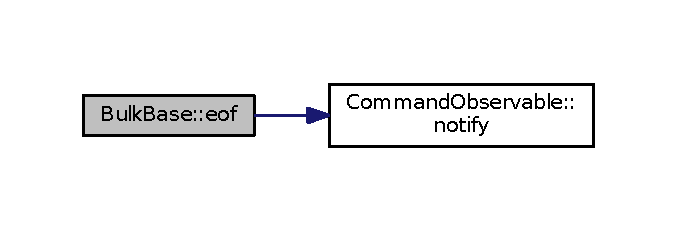
\includegraphics[width=329pt]{class_bulk_base_aff6263fd52d47be936676a1afa890a4a_cgraph}
\end{center}
\end{figure}




Here is the caller graph for this function\+:
\nopagebreak
\begin{figure}[H]
\begin{center}
\leavevmode
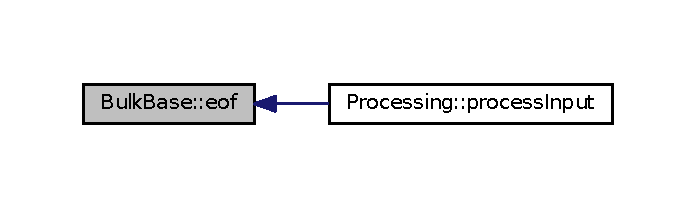
\includegraphics[width=334pt]{class_bulk_base_aff6263fd52d47be936676a1afa890a4a_icgraph}
\end{center}
\end{figure}


\index{Bulk\+Base@{Bulk\+Base}!operator()@{operator()}}
\index{operator()@{operator()}!Bulk\+Base@{Bulk\+Base}}
\subsubsection[{\texorpdfstring{operator()(string \&line)}{operator()(string &line)}}]{\setlength{\rightskip}{0pt plus 5cm}template$<$typename... Out\+Observers$>$ void {\bf Bulk\+Base}$<$ Out\+Observers $>$\+::operator() (
\begin{DoxyParamCaption}
\item[{string \&}]{line}
\end{DoxyParamCaption}
)\hspace{0.3cm}{\ttfamily [inline]}}\hypertarget{class_bulk_base_a3c920e9c377f87728b9d6aaf5116e824}{}\label{class_bulk_base_a3c920e9c377f87728b9d6aaf5116e824}


Definition at line 46 of file bulk.\+h.



The documentation for this class was generated from the following file\+:\begin{DoxyCompactItemize}
\item 
\hyperlink{bulk_8h}{bulk.\+h}\end{DoxyCompactItemize}

\hypertarget{class_cmd_add}{}\section{Cmd\+Add Class Reference}
\label{class_cmd_add}\index{Cmd\+Add@{Cmd\+Add}}


{\ttfamily \#include $<$commands.\+h$>$}



Inheritance diagram for Cmd\+Add\+:
\nopagebreak
\begin{figure}[H]
\begin{center}
\leavevmode
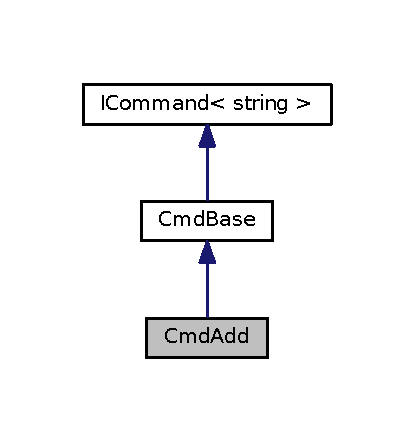
\includegraphics[width=199pt]{class_cmd_add__inherit__graph}
\end{center}
\end{figure}


Collaboration diagram for Cmd\+Add\+:
\nopagebreak
\begin{figure}[H]
\begin{center}
\leavevmode
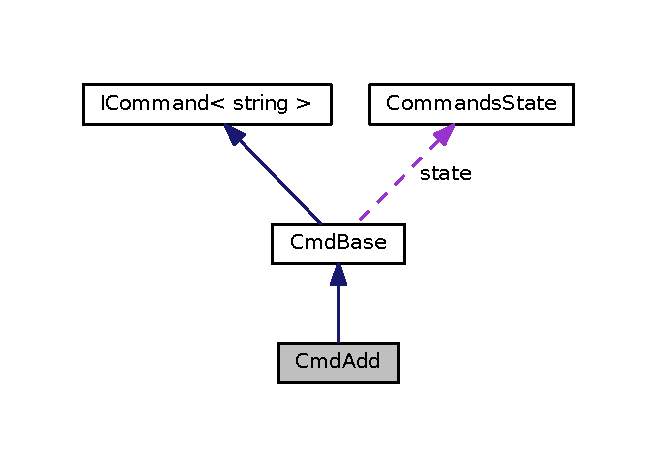
\includegraphics[width=316pt]{class_cmd_add__coll__graph}
\end{center}
\end{figure}
\subsection*{Public Member Functions}
\begin{DoxyCompactItemize}
\item 
void \hyperlink{class_cmd_add_ad68e32ec699775d814a7dc79ebaa5646}{exec} (const string \&data) override
\end{DoxyCompactItemize}
\subsection*{Additional Inherited Members}


\subsection{Detailed Description}


Definition at line 51 of file commands.\+h.



\subsection{Member Function Documentation}
\index{Cmd\+Add@{Cmd\+Add}!exec@{exec}}
\index{exec@{exec}!Cmd\+Add@{Cmd\+Add}}
\subsubsection[{\texorpdfstring{exec(const string \&data) override}{exec(const string &data) override}}]{\setlength{\rightskip}{0pt plus 5cm}void Cmd\+Add\+::exec (
\begin{DoxyParamCaption}
\item[{const string \&}]{data}
\end{DoxyParamCaption}
)\hspace{0.3cm}{\ttfamily [inline]}, {\ttfamily [override]}}\hypertarget{class_cmd_add_ad68e32ec699775d814a7dc79ebaa5646}{}\label{class_cmd_add_ad68e32ec699775d814a7dc79ebaa5646}


Definition at line 53 of file commands.\+h.



Here is the call graph for this function\+:
\nopagebreak
\begin{figure}[H]
\begin{center}
\leavevmode
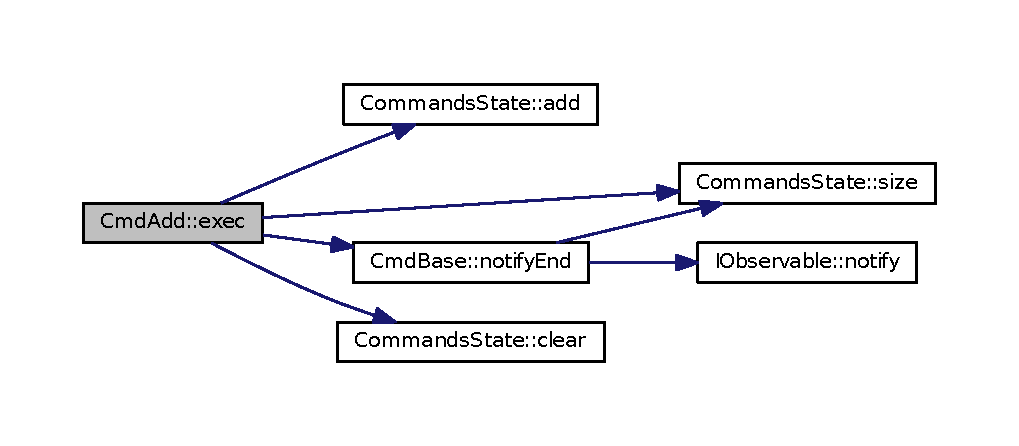
\includegraphics[width=350pt]{class_cmd_add_ad68e32ec699775d814a7dc79ebaa5646_cgraph}
\end{center}
\end{figure}




The documentation for this class was generated from the following file\+:\begin{DoxyCompactItemize}
\item 
\hyperlink{commands_8h}{commands.\+h}\end{DoxyCompactItemize}

\hypertarget{class_cmd_base}{}\section{Cmd\+Base Class Reference}
\label{class_cmd_base}\index{Cmd\+Base@{Cmd\+Base}}


{\ttfamily \#include $<$commands.\+h$>$}



Inheritance diagram for Cmd\+Base\+:
\nopagebreak
\begin{figure}[H]
\begin{center}
\leavevmode
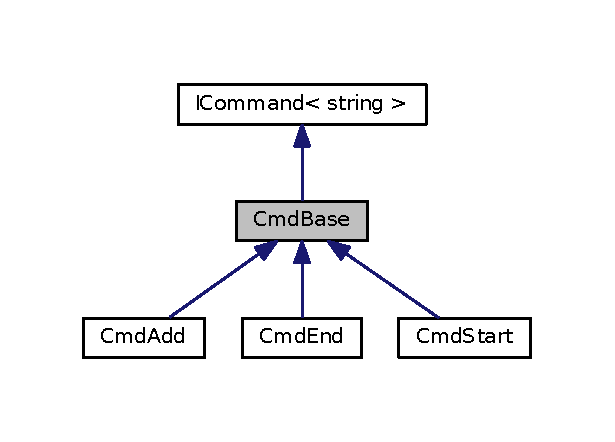
\includegraphics[width=295pt]{class_cmd_base__inherit__graph}
\end{center}
\end{figure}


Collaboration diagram for Cmd\+Base\+:
\nopagebreak
\begin{figure}[H]
\begin{center}
\leavevmode
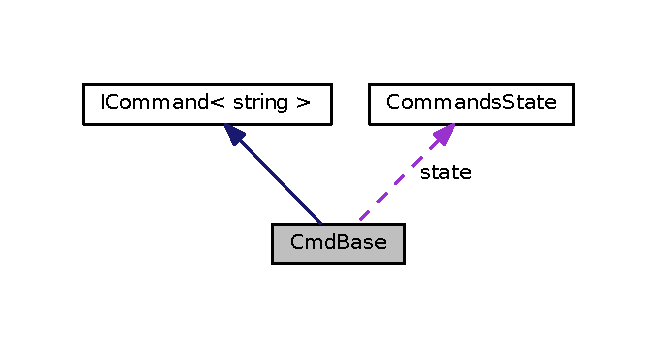
\includegraphics[width=316pt]{class_cmd_base__coll__graph}
\end{center}
\end{figure}
\subsection*{Public Member Functions}
\begin{DoxyCompactItemize}
\item 
void \hyperlink{class_cmd_base_add2802c0ebd8fb70633b83432db0dec2}{init} (\hyperlink{struct_i_observable}{I\+Observable} $\ast$cmd\+Observable, \hyperlink{class_commands_state}{Commands\+State} $\ast$\hyperlink{class_cmd_base_a8960a4214ffcf20763e55b2eb3520a99}{state})
\end{DoxyCompactItemize}
\subsection*{Protected Member Functions}
\begin{DoxyCompactItemize}
\item 
void \hyperlink{class_cmd_base_a090ff153849f8c18e2d0f1182ffa5acd}{notify\+Start} ()
\item 
void \hyperlink{class_cmd_base_a501632bad6f91e45bf8c22073ff432c6}{notify\+End} ()
\item 
void \hyperlink{class_cmd_base_a26df8a46be6e4bb0e9d890a625cdac9d}{notify\+Add} ()
\end{DoxyCompactItemize}
\subsection*{Protected Attributes}
\begin{DoxyCompactItemize}
\item 
\hyperlink{class_commands_state}{Commands\+State} $\ast$ \hyperlink{class_cmd_base_a8960a4214ffcf20763e55b2eb3520a99}{state}
\end{DoxyCompactItemize}


\subsection{Detailed Description}


Definition at line 8 of file commands.\+h.



\subsection{Member Function Documentation}
\index{Cmd\+Base@{Cmd\+Base}!init@{init}}
\index{init@{init}!Cmd\+Base@{Cmd\+Base}}
\subsubsection[{\texorpdfstring{init(\+I\+Observable $\ast$cmd\+Observable, Commands\+State $\ast$state)}{init(IObservable *cmdObservable, CommandsState *state)}}]{\setlength{\rightskip}{0pt plus 5cm}void Cmd\+Base\+::init (
\begin{DoxyParamCaption}
\item[{{\bf I\+Observable} $\ast$}]{cmd\+Observable, }
\item[{{\bf Commands\+State} $\ast$}]{state}
\end{DoxyParamCaption}
)\hspace{0.3cm}{\ttfamily [inline]}}\hypertarget{class_cmd_base_add2802c0ebd8fb70633b83432db0dec2}{}\label{class_cmd_base_add2802c0ebd8fb70633b83432db0dec2}


Definition at line 11 of file commands.\+h.

\index{Cmd\+Base@{Cmd\+Base}!notify\+Add@{notify\+Add}}
\index{notify\+Add@{notify\+Add}!Cmd\+Base@{Cmd\+Base}}
\subsubsection[{\texorpdfstring{notify\+Add()}{notifyAdd()}}]{\setlength{\rightskip}{0pt plus 5cm}void Cmd\+Base\+::notify\+Add (
\begin{DoxyParamCaption}
{}
\end{DoxyParamCaption}
)\hspace{0.3cm}{\ttfamily [inline]}, {\ttfamily [protected]}}\hypertarget{class_cmd_base_a26df8a46be6e4bb0e9d890a625cdac9d}{}\label{class_cmd_base_a26df8a46be6e4bb0e9d890a625cdac9d}


Definition at line 23 of file commands.\+h.



Here is the call graph for this function\+:
\nopagebreak
\begin{figure}[H]
\begin{center}
\leavevmode
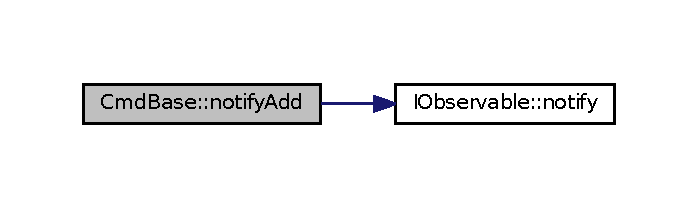
\includegraphics[width=335pt]{class_cmd_base_a26df8a46be6e4bb0e9d890a625cdac9d_cgraph}
\end{center}
\end{figure}


\index{Cmd\+Base@{Cmd\+Base}!notify\+End@{notify\+End}}
\index{notify\+End@{notify\+End}!Cmd\+Base@{Cmd\+Base}}
\subsubsection[{\texorpdfstring{notify\+End()}{notifyEnd()}}]{\setlength{\rightskip}{0pt plus 5cm}void Cmd\+Base\+::notify\+End (
\begin{DoxyParamCaption}
{}
\end{DoxyParamCaption}
)\hspace{0.3cm}{\ttfamily [inline]}, {\ttfamily [protected]}}\hypertarget{class_cmd_base_a501632bad6f91e45bf8c22073ff432c6}{}\label{class_cmd_base_a501632bad6f91e45bf8c22073ff432c6}


Definition at line 20 of file commands.\+h.



Here is the call graph for this function\+:
\nopagebreak
\begin{figure}[H]
\begin{center}
\leavevmode
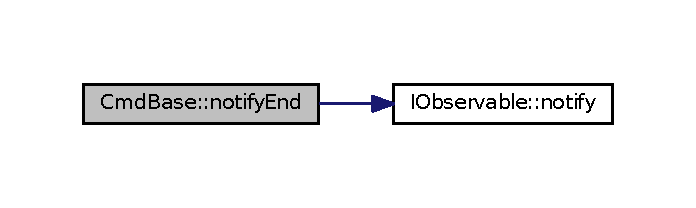
\includegraphics[width=334pt]{class_cmd_base_a501632bad6f91e45bf8c22073ff432c6_cgraph}
\end{center}
\end{figure}




Here is the caller graph for this function\+:
\nopagebreak
\begin{figure}[H]
\begin{center}
\leavevmode
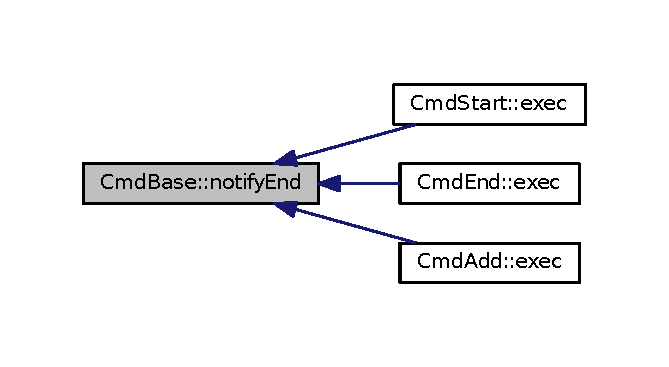
\includegraphics[width=321pt]{class_cmd_base_a501632bad6f91e45bf8c22073ff432c6_icgraph}
\end{center}
\end{figure}


\index{Cmd\+Base@{Cmd\+Base}!notify\+Start@{notify\+Start}}
\index{notify\+Start@{notify\+Start}!Cmd\+Base@{Cmd\+Base}}
\subsubsection[{\texorpdfstring{notify\+Start()}{notifyStart()}}]{\setlength{\rightskip}{0pt plus 5cm}void Cmd\+Base\+::notify\+Start (
\begin{DoxyParamCaption}
{}
\end{DoxyParamCaption}
)\hspace{0.3cm}{\ttfamily [inline]}, {\ttfamily [protected]}}\hypertarget{class_cmd_base_a090ff153849f8c18e2d0f1182ffa5acd}{}\label{class_cmd_base_a090ff153849f8c18e2d0f1182ffa5acd}


Definition at line 17 of file commands.\+h.



Here is the call graph for this function\+:
\nopagebreak
\begin{figure}[H]
\begin{center}
\leavevmode
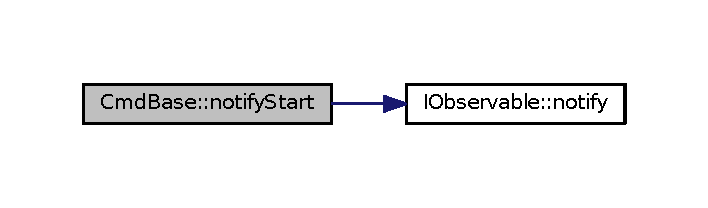
\includegraphics[width=340pt]{class_cmd_base_a090ff153849f8c18e2d0f1182ffa5acd_cgraph}
\end{center}
\end{figure}




Here is the caller graph for this function\+:
\nopagebreak
\begin{figure}[H]
\begin{center}
\leavevmode
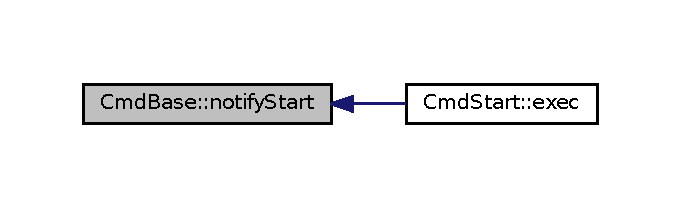
\includegraphics[width=327pt]{class_cmd_base_a090ff153849f8c18e2d0f1182ffa5acd_icgraph}
\end{center}
\end{figure}




\subsection{Member Data Documentation}
\index{Cmd\+Base@{Cmd\+Base}!state@{state}}
\index{state@{state}!Cmd\+Base@{Cmd\+Base}}
\subsubsection[{\texorpdfstring{state}{state}}]{\setlength{\rightskip}{0pt plus 5cm}{\bf Commands\+State}$\ast$ Cmd\+Base\+::state\hspace{0.3cm}{\ttfamily [protected]}}\hypertarget{class_cmd_base_a8960a4214ffcf20763e55b2eb3520a99}{}\label{class_cmd_base_a8960a4214ffcf20763e55b2eb3520a99}


Definition at line 16 of file commands.\+h.



The documentation for this class was generated from the following file\+:\begin{DoxyCompactItemize}
\item 
\hyperlink{commands_8h}{commands.\+h}\end{DoxyCompactItemize}

\hypertarget{class_cmd_end}{}\section{Cmd\+End Class Reference}
\label{class_cmd_end}\index{Cmd\+End@{Cmd\+End}}


{\ttfamily \#include $<$commands.\+h$>$}



Inheritance diagram for Cmd\+End\+:
\nopagebreak
\begin{figure}[H]
\begin{center}
\leavevmode
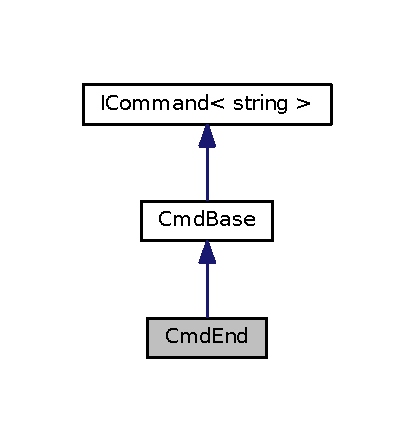
\includegraphics[width=199pt]{class_cmd_end__inherit__graph}
\end{center}
\end{figure}


Collaboration diagram for Cmd\+End\+:
\nopagebreak
\begin{figure}[H]
\begin{center}
\leavevmode
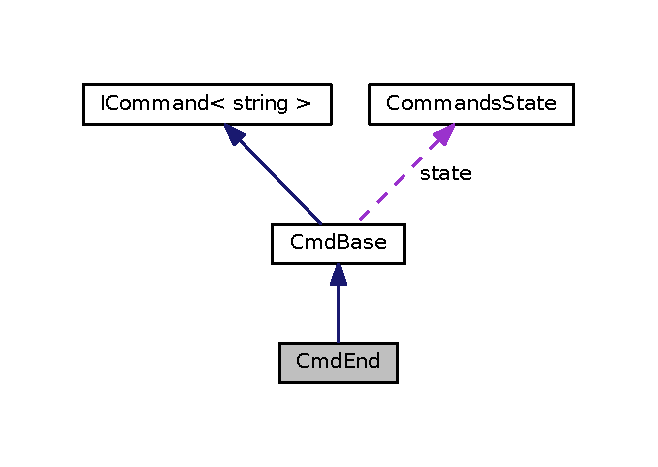
\includegraphics[width=316pt]{class_cmd_end__coll__graph}
\end{center}
\end{figure}
\subsection*{Public Member Functions}
\begin{DoxyCompactItemize}
\item 
void \hyperlink{class_cmd_end_a4c316b96ae2a814838a4c985b8b551ab}{exec} (\mbox{[}\mbox{[}maybe\+\_\+unused\mbox{]}\mbox{]} const string \&data) override
\end{DoxyCompactItemize}
\subsection*{Additional Inherited Members}


\subsection{Detailed Description}


Definition at line 40 of file commands.\+h.



\subsection{Member Function Documentation}
\index{Cmd\+End@{Cmd\+End}!exec@{exec}}
\index{exec@{exec}!Cmd\+End@{Cmd\+End}}
\subsubsection[{\texorpdfstring{exec([[maybe\+\_\+unused]] const string \&data) override}{exec([[maybe_unused]] const string &data) override}}]{\setlength{\rightskip}{0pt plus 5cm}void Cmd\+End\+::exec (
\begin{DoxyParamCaption}
\item[{\mbox{[}\mbox{[}maybe\+\_\+unused\mbox{]} \mbox{]} const string \&}]{data}
\end{DoxyParamCaption}
)\hspace{0.3cm}{\ttfamily [inline]}, {\ttfamily [override]}, {\ttfamily [virtual]}}\hypertarget{class_cmd_end_a4c316b96ae2a814838a4c985b8b551ab}{}\label{class_cmd_end_a4c316b96ae2a814838a4c985b8b551ab}


Implements \hyperlink{struct_i_command_aa00e7af6e23959c4ffef6d990a0750b2}{I\+Command$<$ string $>$}.



Definition at line 42 of file commands.\+h.



Here is the call graph for this function\+:
\nopagebreak
\begin{figure}[H]
\begin{center}
\leavevmode
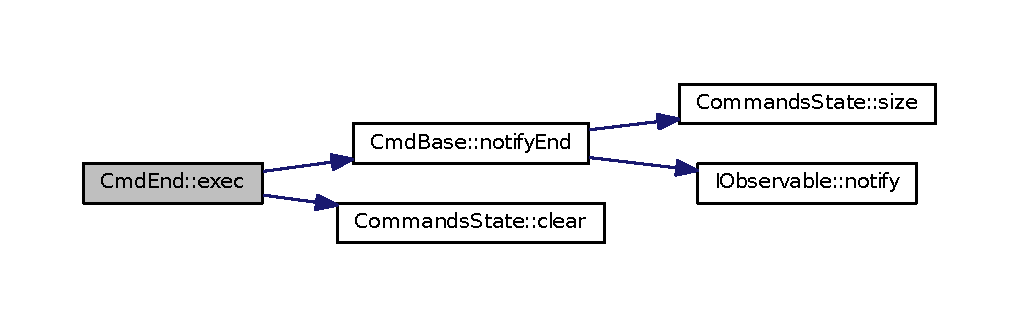
\includegraphics[width=350pt]{class_cmd_end_a4c316b96ae2a814838a4c985b8b551ab_cgraph}
\end{center}
\end{figure}




The documentation for this class was generated from the following file\+:\begin{DoxyCompactItemize}
\item 
\hyperlink{commands_8h}{commands.\+h}\end{DoxyCompactItemize}

\hypertarget{class_cmd_start}{}\section{Cmd\+Start Class Reference}
\label{class_cmd_start}\index{Cmd\+Start@{Cmd\+Start}}


{\ttfamily \#include $<$commands.\+h$>$}



Inheritance diagram for Cmd\+Start\+:
\nopagebreak
\begin{figure}[H]
\begin{center}
\leavevmode
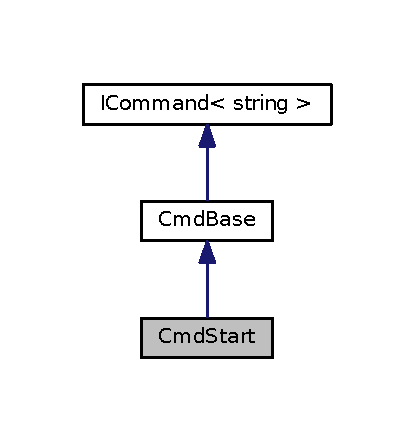
\includegraphics[width=199pt]{class_cmd_start__inherit__graph}
\end{center}
\end{figure}


Collaboration diagram for Cmd\+Start\+:
\nopagebreak
\begin{figure}[H]
\begin{center}
\leavevmode
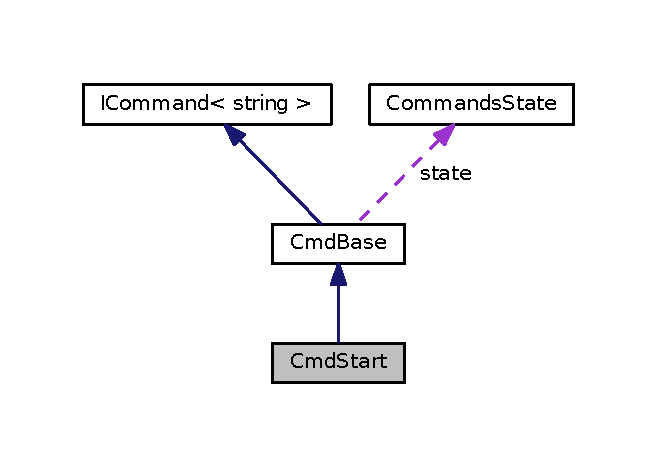
\includegraphics[width=316pt]{class_cmd_start__coll__graph}
\end{center}
\end{figure}
\subsection*{Public Member Functions}
\begin{DoxyCompactItemize}
\item 
void \hyperlink{class_cmd_start_acf20f86d72982205d1af586b5e09846e}{exec} (\mbox{[}\mbox{[}maybe\+\_\+unused\mbox{]}\mbox{]} const string \&data) override
\end{DoxyCompactItemize}
\subsection*{Additional Inherited Members}


\subsection{Detailed Description}


Definition at line 28 of file commands.\+h.



\subsection{Member Function Documentation}
\index{Cmd\+Start@{Cmd\+Start}!exec@{exec}}
\index{exec@{exec}!Cmd\+Start@{Cmd\+Start}}
\subsubsection[{\texorpdfstring{exec([[maybe\+\_\+unused]] const string \&data) override}{exec([[maybe_unused]] const string &data) override}}]{\setlength{\rightskip}{0pt plus 5cm}void Cmd\+Start\+::exec (
\begin{DoxyParamCaption}
\item[{\mbox{[}\mbox{[}maybe\+\_\+unused\mbox{]} \mbox{]} const string \&}]{data}
\end{DoxyParamCaption}
)\hspace{0.3cm}{\ttfamily [inline]}, {\ttfamily [override]}, {\ttfamily [virtual]}}\hypertarget{class_cmd_start_acf20f86d72982205d1af586b5e09846e}{}\label{class_cmd_start_acf20f86d72982205d1af586b5e09846e}


Implements \hyperlink{struct_i_command_aa00e7af6e23959c4ffef6d990a0750b2}{I\+Command$<$ string $>$}.



Definition at line 30 of file commands.\+h.



Here is the call graph for this function\+:
\nopagebreak
\begin{figure}[H]
\begin{center}
\leavevmode
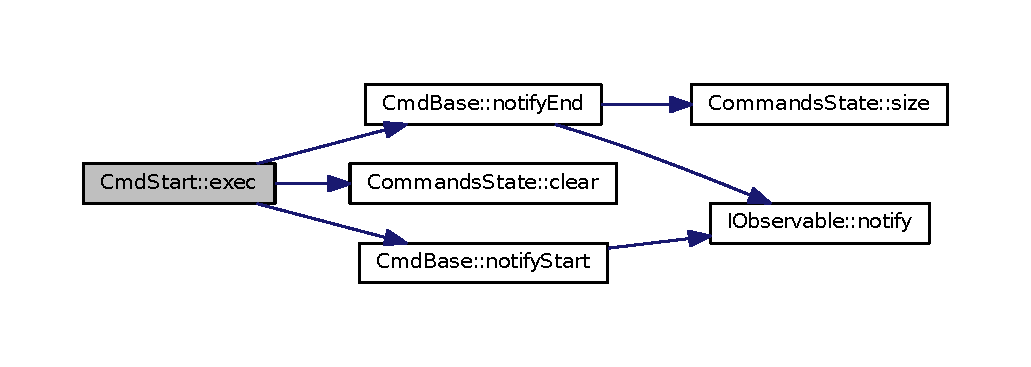
\includegraphics[width=350pt]{class_cmd_start_acf20f86d72982205d1af586b5e09846e_cgraph}
\end{center}
\end{figure}




The documentation for this class was generated from the following file\+:\begin{DoxyCompactItemize}
\item 
\hyperlink{commands_8h}{commands.\+h}\end{DoxyCompactItemize}

\hypertarget{struct_collector_observer}{}\section{Collector\+Observer Struct Reference}
\label{struct_collector_observer}\index{Collector\+Observer@{Collector\+Observer}}


{\ttfamily \#include $<$observers.\+h$>$}



Inheritance diagram for Collector\+Observer\+:
\nopagebreak
\begin{figure}[H]
\begin{center}
\leavevmode
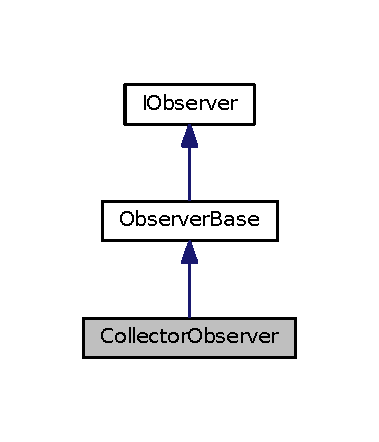
\includegraphics[width=182pt]{struct_collector_observer__inherit__graph}
\end{center}
\end{figure}


Collaboration diagram for Collector\+Observer\+:
\nopagebreak
\begin{figure}[H]
\begin{center}
\leavevmode
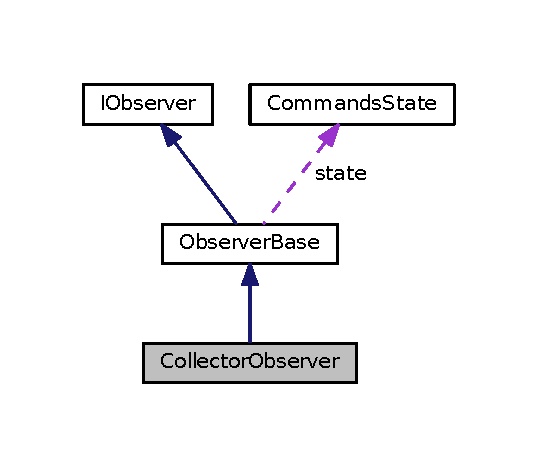
\includegraphics[width=258pt]{struct_collector_observer__coll__graph}
\end{center}
\end{figure}
\subsection*{Public Member Functions}
\begin{DoxyCompactItemize}
\item 
\hyperlink{struct_collector_observer_a1bd761e7bb5cd7787c2496ad3cc3e465}{Collector\+Observer} (\hyperlink{struct_i_observable}{I\+Observable} \&observable, \hyperlink{class_commands_state}{Commands\+State} \&\hyperlink{struct_observer_base_a107ad54040309605fa5fafd481b97f2f}{state})
\item 
void \hyperlink{struct_collector_observer_adebc5768f5778ceb3e981362363db247}{update} (\hyperlink{interface_8h_aa299181f275f76f11365a410f7429098}{E\+Command} cmd, string data)
\end{DoxyCompactItemize}
\subsection*{Additional Inherited Members}


\subsection{Detailed Description}


Definition at line 34 of file observers.\+h.



\subsection{Constructor \& Destructor Documentation}
\index{Collector\+Observer@{Collector\+Observer}!Collector\+Observer@{Collector\+Observer}}
\index{Collector\+Observer@{Collector\+Observer}!Collector\+Observer@{Collector\+Observer}}
\subsubsection[{\texorpdfstring{Collector\+Observer(\+I\+Observable \&observable, Commands\+State \&state)}{CollectorObserver(IObservable &observable, CommandsState &state)}}]{\setlength{\rightskip}{0pt plus 5cm}Collector\+Observer\+::\+Collector\+Observer (
\begin{DoxyParamCaption}
\item[{{\bf I\+Observable} \&}]{observable, }
\item[{{\bf Commands\+State} \&}]{state}
\end{DoxyParamCaption}
)\hspace{0.3cm}{\ttfamily [inline]}}\hypertarget{struct_collector_observer_a1bd761e7bb5cd7787c2496ad3cc3e465}{}\label{struct_collector_observer_a1bd761e7bb5cd7787c2496ad3cc3e465}


Definition at line 35 of file observers.\+h.



\subsection{Member Function Documentation}
\index{Collector\+Observer@{Collector\+Observer}!update@{update}}
\index{update@{update}!Collector\+Observer@{Collector\+Observer}}
\subsubsection[{\texorpdfstring{update(\+E\+Command cmd, string data)}{update(ECommand cmd, string data)}}]{\setlength{\rightskip}{0pt plus 5cm}void Collector\+Observer\+::update (
\begin{DoxyParamCaption}
\item[{{\bf E\+Command}}]{cmd, }
\item[{string}]{data}
\end{DoxyParamCaption}
)\hspace{0.3cm}{\ttfamily [inline]}, {\ttfamily [virtual]}}\hypertarget{struct_collector_observer_adebc5768f5778ceb3e981362363db247}{}\label{struct_collector_observer_adebc5768f5778ceb3e981362363db247}


Implements \hyperlink{struct_i_observer_a87304ed05adacf4219c5e4252629ae14}{I\+Observer}.



Definition at line 36 of file observers.\+h.



Here is the call graph for this function\+:
\nopagebreak
\begin{figure}[H]
\begin{center}
\leavevmode
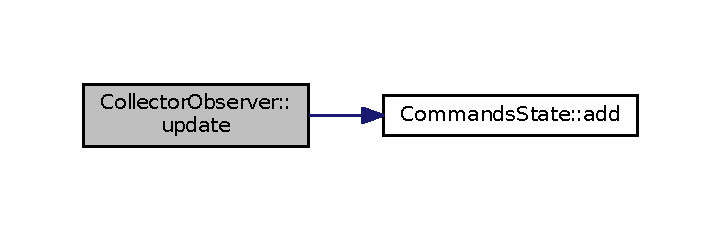
\includegraphics[width=346pt]{struct_collector_observer_adebc5768f5778ceb3e981362363db247_cgraph}
\end{center}
\end{figure}




The documentation for this struct was generated from the following file\+:\begin{DoxyCompactItemize}
\item 
\hyperlink{observers_8h}{observers.\+h}\end{DoxyCompactItemize}

\hypertarget{class_command_observable}{}\section{Command\+Observable Class Reference}
\label{class_command_observable}\index{Command\+Observable@{Command\+Observable}}


{\ttfamily \#include $<$state.\+h$>$}



Inheritance diagram for Command\+Observable\+:
\nopagebreak
\begin{figure}[H]
\begin{center}
\leavevmode
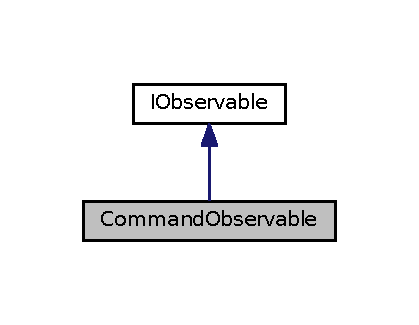
\includegraphics[width=201pt]{class_command_observable__inherit__graph}
\end{center}
\end{figure}


Collaboration diagram for Command\+Observable\+:
\nopagebreak
\begin{figure}[H]
\begin{center}
\leavevmode
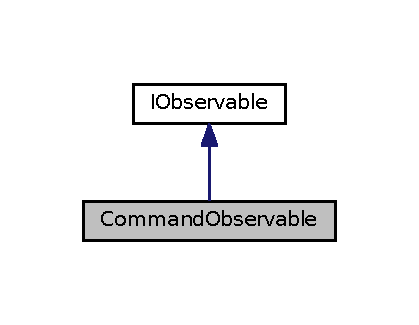
\includegraphics[width=201pt]{class_command_observable__coll__graph}
\end{center}
\end{figure}
\subsection*{Public Member Functions}
\begin{DoxyCompactItemize}
\item 
void \hyperlink{class_command_observable_ad8bc68d264feb6c62ba2964e57c7c1ac}{subscribe} (\hyperlink{struct_i_observer}{I\+Observer} $\ast$observer) override
\item 
void \hyperlink{class_command_observable_a6df1f72513d0964125e6eec93a861335}{notify} (\hyperlink{interface_8h_aa299181f275f76f11365a410f7429098}{E\+Command} cmd) override
\item 
void \hyperlink{class_command_observable_ae1da1f83ac5b27fc0d6dbaa5dd1e773b}{notify} (\hyperlink{interface_8h_aa299181f275f76f11365a410f7429098}{E\+Command} cmd, string data) override
\end{DoxyCompactItemize}


\subsection{Detailed Description}


Definition at line 50 of file state.\+h.



\subsection{Member Function Documentation}
\index{Command\+Observable@{Command\+Observable}!notify@{notify}}
\index{notify@{notify}!Command\+Observable@{Command\+Observable}}
\subsubsection[{\texorpdfstring{notify(\+E\+Command cmd) override}{notify(ECommand cmd) override}}]{\setlength{\rightskip}{0pt plus 5cm}void Command\+Observable\+::notify (
\begin{DoxyParamCaption}
\item[{{\bf E\+Command}}]{cmd}
\end{DoxyParamCaption}
)\hspace{0.3cm}{\ttfamily [inline]}, {\ttfamily [override]}, {\ttfamily [virtual]}}\hypertarget{class_command_observable_a6df1f72513d0964125e6eec93a861335}{}\label{class_command_observable_a6df1f72513d0964125e6eec93a861335}


Implements \hyperlink{struct_i_observable_a639f160d68e626515e6d977f813c3b09}{I\+Observable}.



Definition at line 56 of file state.\+h.

\index{Command\+Observable@{Command\+Observable}!notify@{notify}}
\index{notify@{notify}!Command\+Observable@{Command\+Observable}}
\subsubsection[{\texorpdfstring{notify(\+E\+Command cmd, string data) override}{notify(ECommand cmd, string data) override}}]{\setlength{\rightskip}{0pt plus 5cm}void Command\+Observable\+::notify (
\begin{DoxyParamCaption}
\item[{{\bf E\+Command}}]{cmd, }
\item[{string}]{data}
\end{DoxyParamCaption}
)\hspace{0.3cm}{\ttfamily [inline]}, {\ttfamily [override]}}\hypertarget{class_command_observable_ae1da1f83ac5b27fc0d6dbaa5dd1e773b}{}\label{class_command_observable_ae1da1f83ac5b27fc0d6dbaa5dd1e773b}


Definition at line 61 of file state.\+h.

\index{Command\+Observable@{Command\+Observable}!subscribe@{subscribe}}
\index{subscribe@{subscribe}!Command\+Observable@{Command\+Observable}}
\subsubsection[{\texorpdfstring{subscribe(\+I\+Observer $\ast$observer) override}{subscribe(IObserver *observer) override}}]{\setlength{\rightskip}{0pt plus 5cm}void Command\+Observable\+::subscribe (
\begin{DoxyParamCaption}
\item[{{\bf I\+Observer} $\ast$}]{observer}
\end{DoxyParamCaption}
)\hspace{0.3cm}{\ttfamily [inline]}, {\ttfamily [override]}, {\ttfamily [virtual]}}\hypertarget{class_command_observable_ad8bc68d264feb6c62ba2964e57c7c1ac}{}\label{class_command_observable_ad8bc68d264feb6c62ba2964e57c7c1ac}


Implements \hyperlink{struct_i_observable_a20ae9c2f2d4618af71f8eae770f2cadd}{I\+Observable}.



Definition at line 53 of file state.\+h.



The documentation for this class was generated from the following file\+:\begin{DoxyCompactItemize}
\item 
\hyperlink{state_8h}{state.\+h}\end{DoxyCompactItemize}

\hypertarget{class_commands_handler}{}\section{Commands\+Handler Class Reference}
\label{class_commands_handler}\index{Commands\+Handler@{Commands\+Handler}}


{\ttfamily \#include $<$commands.\+h$>$}

\subsection*{Public Member Functions}
\begin{DoxyCompactItemize}
\item 
\hyperlink{class_commands_handler_a97bcb79d779c084ac1d7f8fbe327a70f}{Commands\+Handler} (\hyperlink{struct_i_observable}{I\+Observable} \&observable, \hyperlink{class_commands_state}{Commands\+State} \&state)
\item 
void \hyperlink{class_commands_handler_a01d015d93967a927d4989f4f3a8f4a18}{operator()} (string \&line)
\item 
void \hyperlink{class_commands_handler_a1673afa4a00e96c0b1515c3478768b85}{eof} ()
\end{DoxyCompactItemize}


\subsection{Detailed Description}


Definition at line 76 of file commands.\+h.



\subsection{Constructor \& Destructor Documentation}
\index{Commands\+Handler@{Commands\+Handler}!Commands\+Handler@{Commands\+Handler}}
\index{Commands\+Handler@{Commands\+Handler}!Commands\+Handler@{Commands\+Handler}}
\subsubsection[{\texorpdfstring{Commands\+Handler(\+I\+Observable \&observable, Commands\+State \&state)}{CommandsHandler(IObservable &observable, CommandsState &state)}}]{\setlength{\rightskip}{0pt plus 5cm}Commands\+Handler\+::\+Commands\+Handler (
\begin{DoxyParamCaption}
\item[{{\bf I\+Observable} \&}]{observable, }
\item[{{\bf Commands\+State} \&}]{state}
\end{DoxyParamCaption}
)\hspace{0.3cm}{\ttfamily [inline]}}\hypertarget{class_commands_handler_a97bcb79d779c084ac1d7f8fbe327a70f}{}\label{class_commands_handler_a97bcb79d779c084ac1d7f8fbe327a70f}


Definition at line 88 of file commands.\+h.



\subsection{Member Function Documentation}
\index{Commands\+Handler@{Commands\+Handler}!eof@{eof}}
\index{eof@{eof}!Commands\+Handler@{Commands\+Handler}}
\subsubsection[{\texorpdfstring{eof()}{eof()}}]{\setlength{\rightskip}{0pt plus 5cm}void Commands\+Handler\+::eof (
\begin{DoxyParamCaption}
{}
\end{DoxyParamCaption}
)\hspace{0.3cm}{\ttfamily [inline]}}\hypertarget{class_commands_handler_a1673afa4a00e96c0b1515c3478768b85}{}\label{class_commands_handler_a1673afa4a00e96c0b1515c3478768b85}


Definition at line 106 of file commands.\+h.



Here is the caller graph for this function\+:
\nopagebreak
\begin{figure}[H]
\begin{center}
\leavevmode
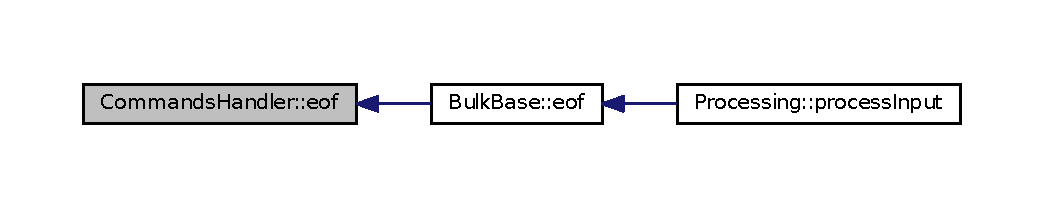
\includegraphics[width=350pt]{class_commands_handler_a1673afa4a00e96c0b1515c3478768b85_icgraph}
\end{center}
\end{figure}


\index{Commands\+Handler@{Commands\+Handler}!operator()@{operator()}}
\index{operator()@{operator()}!Commands\+Handler@{Commands\+Handler}}
\subsubsection[{\texorpdfstring{operator()(string \&line)}{operator()(string &line)}}]{\setlength{\rightskip}{0pt plus 5cm}void Commands\+Handler\+::operator() (
\begin{DoxyParamCaption}
\item[{string \&}]{line}
\end{DoxyParamCaption}
)\hspace{0.3cm}{\ttfamily [inline]}}\hypertarget{class_commands_handler_a01d015d93967a927d4989f4f3a8f4a18}{}\label{class_commands_handler_a01d015d93967a927d4989f4f3a8f4a18}


Definition at line 94 of file commands.\+h.



The documentation for this class was generated from the following file\+:\begin{DoxyCompactItemize}
\item 
\hyperlink{commands_8h}{commands.\+h}\end{DoxyCompactItemize}

\hypertarget{class_commands_state}{}\section{Commands\+State Class Reference}
\label{class_commands_state}\index{Commands\+State@{Commands\+State}}


{\ttfamily \#include $<$state.\+h$>$}

\subsection*{Public Member Functions}
\begin{DoxyCompactItemize}
\item 
void \hyperlink{class_commands_state_a30081a551862ef539927f368fd729d1b}{init} (int \hyperlink{class_commands_state_ae3cbeca97ad210a6980d5c44cf6adee2}{limit})
\item 
void \hyperlink{class_commands_state_abd5de3a66178e6a7bead6ca7ff3bd1c3}{add} (const string \&cmdline)
\item 
void \hyperlink{class_commands_state_ae19501ca13fe9e1c5ebebe73eeaf8f72}{remove\+Last} ()
\item 
void \hyperlink{class_commands_state_a1cab17d80f32092592c5d863efe3a610}{for\+Each} (std\+::function$<$ void(string \&cmd)$>$ fn)
\item 
void \hyperlink{class_commands_state_a15f9a11035f9efddb3ea023a9fb63b61}{for\+Each} (std\+::function$<$ void(string \&cmd, bool is\+First, bool is\+Last)$>$ fn)
\item 
void \hyperlink{class_commands_state_a638034095963268ab56211c2933fddac}{clear} ()
\item 
string \& \hyperlink{class_commands_state_a55a67a2f27e9b500a993242b5e808d96}{get\+Last} ()
\item 
size\+\_\+t \hyperlink{class_commands_state_a74ea73a7753aee71cfdacb8ac0fc7ad7}{size} ()
\end{DoxyCompactItemize}
\subsection*{Public Attributes}
\begin{DoxyCompactItemize}
\item 
unsigned \hyperlink{class_commands_state_ae3cbeca97ad210a6980d5c44cf6adee2}{limit} = 0
\item 
unsigned \hyperlink{class_commands_state_a9d4a6edd6fc21c07150ec1bebf8516f4}{new\+Count} = 0
\item 
std\+::time\+\_\+t \hyperlink{class_commands_state_affdc3152f2776d90a04971104fea81af}{start\+\_\+read} = 0
\end{DoxyCompactItemize}


\subsection{Detailed Description}


Definition at line 13 of file state.\+h.



\subsection{Member Function Documentation}
\index{Commands\+State@{Commands\+State}!add@{add}}
\index{add@{add}!Commands\+State@{Commands\+State}}
\subsubsection[{\texorpdfstring{add(const string \&cmdline)}{add(const string &cmdline)}}]{\setlength{\rightskip}{0pt plus 5cm}void Commands\+State\+::add (
\begin{DoxyParamCaption}
\item[{const string \&}]{cmdline}
\end{DoxyParamCaption}
)\hspace{0.3cm}{\ttfamily [inline]}}\hypertarget{class_commands_state_abd5de3a66178e6a7bead6ca7ff3bd1c3}{}\label{class_commands_state_abd5de3a66178e6a7bead6ca7ff3bd1c3}


Definition at line 20 of file state.\+h.



Here is the caller graph for this function\+:
\nopagebreak
\begin{figure}[H]
\begin{center}
\leavevmode
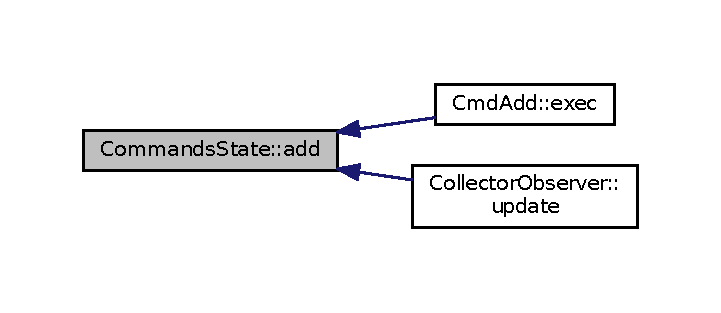
\includegraphics[width=346pt]{class_commands_state_abd5de3a66178e6a7bead6ca7ff3bd1c3_icgraph}
\end{center}
\end{figure}


\index{Commands\+State@{Commands\+State}!clear@{clear}}
\index{clear@{clear}!Commands\+State@{Commands\+State}}
\subsubsection[{\texorpdfstring{clear()}{clear()}}]{\setlength{\rightskip}{0pt plus 5cm}void Commands\+State\+::clear (
\begin{DoxyParamCaption}
{}
\end{DoxyParamCaption}
)\hspace{0.3cm}{\ttfamily [inline]}}\hypertarget{class_commands_state_a638034095963268ab56211c2933fddac}{}\label{class_commands_state_a638034095963268ab56211c2933fddac}


Definition at line 39 of file state.\+h.



Here is the caller graph for this function\+:
\nopagebreak
\begin{figure}[H]
\begin{center}
\leavevmode
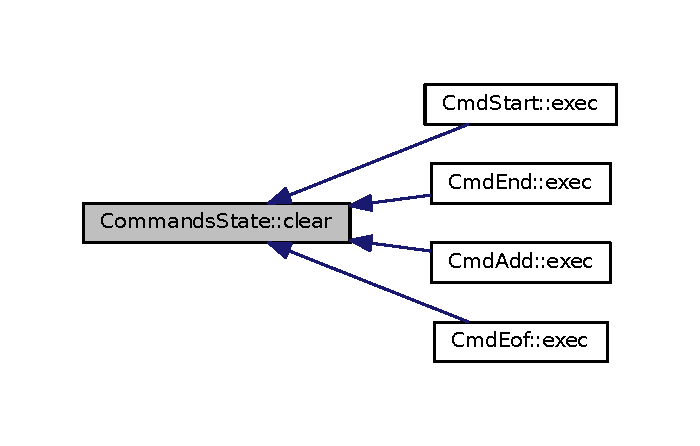
\includegraphics[width=336pt]{class_commands_state_a638034095963268ab56211c2933fddac_icgraph}
\end{center}
\end{figure}


\index{Commands\+State@{Commands\+State}!for\+Each@{for\+Each}}
\index{for\+Each@{for\+Each}!Commands\+State@{Commands\+State}}
\subsubsection[{\texorpdfstring{for\+Each(std\+::function$<$ void(string \&cmd)$>$ fn)}{forEach(std::function< void(string &cmd)> fn)}}]{\setlength{\rightskip}{0pt plus 5cm}void Commands\+State\+::for\+Each (
\begin{DoxyParamCaption}
\item[{std\+::function$<$ void(string \&cmd)$>$}]{fn}
\end{DoxyParamCaption}
)\hspace{0.3cm}{\ttfamily [inline]}}\hypertarget{class_commands_state_a1cab17d80f32092592c5d863efe3a610}{}\label{class_commands_state_a1cab17d80f32092592c5d863efe3a610}


Definition at line 29 of file state.\+h.



Here is the caller graph for this function\+:
\nopagebreak
\begin{figure}[H]
\begin{center}
\leavevmode
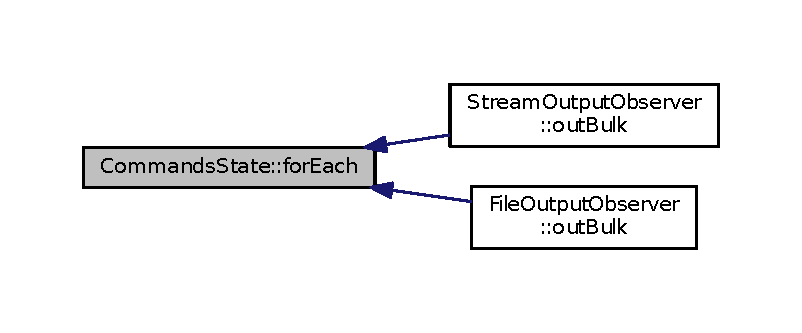
\includegraphics[width=350pt]{class_commands_state_a1cab17d80f32092592c5d863efe3a610_icgraph}
\end{center}
\end{figure}


\index{Commands\+State@{Commands\+State}!for\+Each@{for\+Each}}
\index{for\+Each@{for\+Each}!Commands\+State@{Commands\+State}}
\subsubsection[{\texorpdfstring{for\+Each(std\+::function$<$ void(string \&cmd, bool is\+First, bool is\+Last)$>$ fn)}{forEach(std::function< void(string &cmd, bool isFirst, bool isLast)> fn)}}]{\setlength{\rightskip}{0pt plus 5cm}void Commands\+State\+::for\+Each (
\begin{DoxyParamCaption}
\item[{std\+::function$<$ void(string \&cmd, bool is\+First, bool is\+Last)$>$}]{fn}
\end{DoxyParamCaption}
)\hspace{0.3cm}{\ttfamily [inline]}}\hypertarget{class_commands_state_a15f9a11035f9efddb3ea023a9fb63b61}{}\label{class_commands_state_a15f9a11035f9efddb3ea023a9fb63b61}


Definition at line 32 of file state.\+h.



Here is the call graph for this function\+:
\nopagebreak
\begin{figure}[H]
\begin{center}
\leavevmode
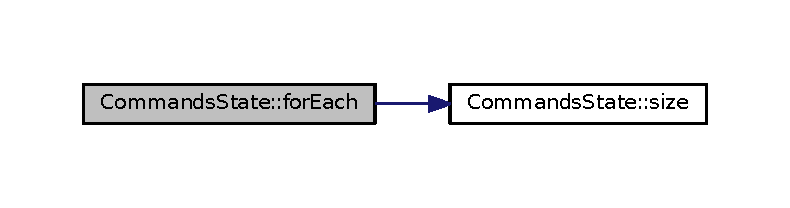
\includegraphics[width=350pt]{class_commands_state_a15f9a11035f9efddb3ea023a9fb63b61_cgraph}
\end{center}
\end{figure}


\index{Commands\+State@{Commands\+State}!get\+Last@{get\+Last}}
\index{get\+Last@{get\+Last}!Commands\+State@{Commands\+State}}
\subsubsection[{\texorpdfstring{get\+Last()}{getLast()}}]{\setlength{\rightskip}{0pt plus 5cm}string\& Commands\+State\+::get\+Last (
\begin{DoxyParamCaption}
{}
\end{DoxyParamCaption}
)\hspace{0.3cm}{\ttfamily [inline]}}\hypertarget{class_commands_state_a55a67a2f27e9b500a993242b5e808d96}{}\label{class_commands_state_a55a67a2f27e9b500a993242b5e808d96}


Definition at line 44 of file state.\+h.

\index{Commands\+State@{Commands\+State}!init@{init}}
\index{init@{init}!Commands\+State@{Commands\+State}}
\subsubsection[{\texorpdfstring{init(int limit)}{init(int limit)}}]{\setlength{\rightskip}{0pt plus 5cm}void Commands\+State\+::init (
\begin{DoxyParamCaption}
\item[{int}]{limit}
\end{DoxyParamCaption}
)\hspace{0.3cm}{\ttfamily [inline]}}\hypertarget{class_commands_state_a30081a551862ef539927f368fd729d1b}{}\label{class_commands_state_a30081a551862ef539927f368fd729d1b}


Definition at line 19 of file state.\+h.

\index{Commands\+State@{Commands\+State}!remove\+Last@{remove\+Last}}
\index{remove\+Last@{remove\+Last}!Commands\+State@{Commands\+State}}
\subsubsection[{\texorpdfstring{remove\+Last()}{removeLast()}}]{\setlength{\rightskip}{0pt plus 5cm}void Commands\+State\+::remove\+Last (
\begin{DoxyParamCaption}
{}
\end{DoxyParamCaption}
)\hspace{0.3cm}{\ttfamily [inline]}}\hypertarget{class_commands_state_ae19501ca13fe9e1c5ebebe73eeaf8f72}{}\label{class_commands_state_ae19501ca13fe9e1c5ebebe73eeaf8f72}


Definition at line 26 of file state.\+h.

\index{Commands\+State@{Commands\+State}!size@{size}}
\index{size@{size}!Commands\+State@{Commands\+State}}
\subsubsection[{\texorpdfstring{size()}{size()}}]{\setlength{\rightskip}{0pt plus 5cm}size\+\_\+t Commands\+State\+::size (
\begin{DoxyParamCaption}
{}
\end{DoxyParamCaption}
)\hspace{0.3cm}{\ttfamily [inline]}}\hypertarget{class_commands_state_a74ea73a7753aee71cfdacb8ac0fc7ad7}{}\label{class_commands_state_a74ea73a7753aee71cfdacb8ac0fc7ad7}


Definition at line 47 of file state.\+h.



Here is the caller graph for this function\+:
\nopagebreak
\begin{figure}[H]
\begin{center}
\leavevmode
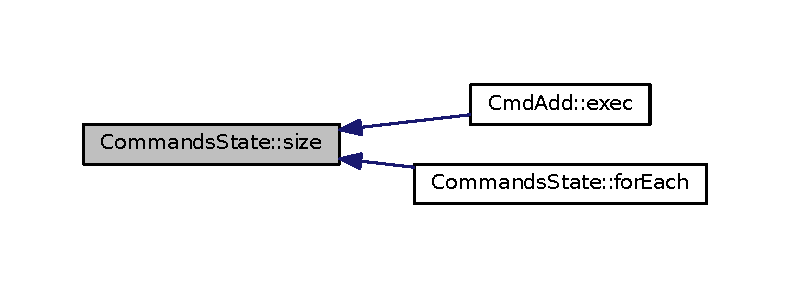
\includegraphics[width=350pt]{class_commands_state_a74ea73a7753aee71cfdacb8ac0fc7ad7_icgraph}
\end{center}
\end{figure}




\subsection{Member Data Documentation}
\index{Commands\+State@{Commands\+State}!limit@{limit}}
\index{limit@{limit}!Commands\+State@{Commands\+State}}
\subsubsection[{\texorpdfstring{limit}{limit}}]{\setlength{\rightskip}{0pt plus 5cm}unsigned Commands\+State\+::limit = 0}\hypertarget{class_commands_state_ae3cbeca97ad210a6980d5c44cf6adee2}{}\label{class_commands_state_ae3cbeca97ad210a6980d5c44cf6adee2}


Definition at line 16 of file state.\+h.

\index{Commands\+State@{Commands\+State}!new\+Count@{new\+Count}}
\index{new\+Count@{new\+Count}!Commands\+State@{Commands\+State}}
\subsubsection[{\texorpdfstring{new\+Count}{newCount}}]{\setlength{\rightskip}{0pt plus 5cm}unsigned Commands\+State\+::new\+Count = 0}\hypertarget{class_commands_state_a9d4a6edd6fc21c07150ec1bebf8516f4}{}\label{class_commands_state_a9d4a6edd6fc21c07150ec1bebf8516f4}


Definition at line 17 of file state.\+h.

\index{Commands\+State@{Commands\+State}!start\+\_\+read@{start\+\_\+read}}
\index{start\+\_\+read@{start\+\_\+read}!Commands\+State@{Commands\+State}}
\subsubsection[{\texorpdfstring{start\+\_\+read}{start_read}}]{\setlength{\rightskip}{0pt plus 5cm}std\+::time\+\_\+t Commands\+State\+::start\+\_\+read = 0}\hypertarget{class_commands_state_affdc3152f2776d90a04971104fea81af}{}\label{class_commands_state_affdc3152f2776d90a04971104fea81af}


Definition at line 18 of file state.\+h.



The documentation for this class was generated from the following file\+:\begin{DoxyCompactItemize}
\item 
\hyperlink{state_8h}{state.\+h}\end{DoxyCompactItemize}

\hypertarget{struct_console_output_observer}{}\section{Console\+Output\+Observer Struct Reference}
\label{struct_console_output_observer}\index{Console\+Output\+Observer@{Console\+Output\+Observer}}


{\ttfamily \#include $<$observers.\+h$>$}



Inheritance diagram for Console\+Output\+Observer\+:
\nopagebreak
\begin{figure}[H]
\begin{center}
\leavevmode
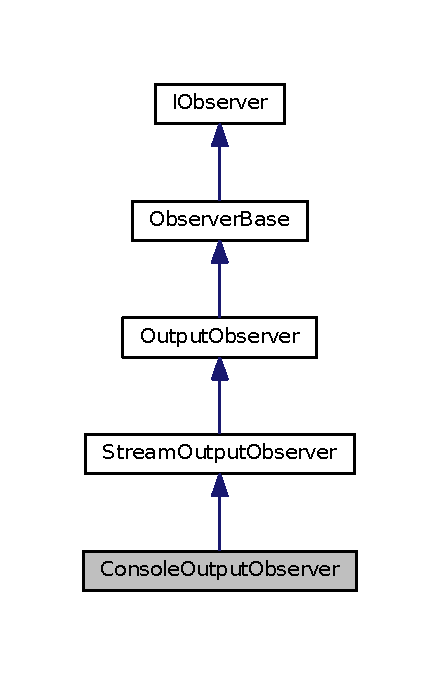
\includegraphics[width=211pt]{struct_console_output_observer__inherit__graph}
\end{center}
\end{figure}


Collaboration diagram for Console\+Output\+Observer\+:
\nopagebreak
\begin{figure}[H]
\begin{center}
\leavevmode
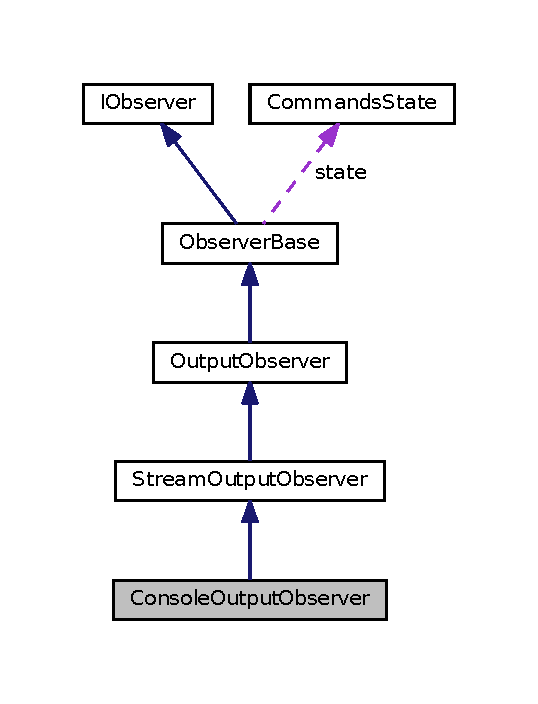
\includegraphics[width=258pt]{struct_console_output_observer__coll__graph}
\end{center}
\end{figure}
\subsection*{Public Member Functions}
\begin{DoxyCompactItemize}
\item 
\hyperlink{struct_console_output_observer_a4f4f1abf132c680b2f0913183d089f08}{Console\+Output\+Observer} (\hyperlink{struct_i_observable}{I\+Observable} \&observable, \hyperlink{class_commands_state}{Commands\+State} \&\hyperlink{struct_observer_base_a107ad54040309605fa5fafd481b97f2f}{state})
\end{DoxyCompactItemize}
\subsection*{Additional Inherited Members}


\subsection{Detailed Description}


Definition at line 76 of file observers.\+h.



\subsection{Constructor \& Destructor Documentation}
\index{Console\+Output\+Observer@{Console\+Output\+Observer}!Console\+Output\+Observer@{Console\+Output\+Observer}}
\index{Console\+Output\+Observer@{Console\+Output\+Observer}!Console\+Output\+Observer@{Console\+Output\+Observer}}
\subsubsection[{\texorpdfstring{Console\+Output\+Observer(\+I\+Observable \&observable, Commands\+State \&state)}{ConsoleOutputObserver(IObservable &observable, CommandsState &state)}}]{\setlength{\rightskip}{0pt plus 5cm}Console\+Output\+Observer\+::\+Console\+Output\+Observer (
\begin{DoxyParamCaption}
\item[{{\bf I\+Observable} \&}]{observable, }
\item[{{\bf Commands\+State} \&}]{state}
\end{DoxyParamCaption}
)\hspace{0.3cm}{\ttfamily [inline]}}\hypertarget{struct_console_output_observer_a4f4f1abf132c680b2f0913183d089f08}{}\label{struct_console_output_observer_a4f4f1abf132c680b2f0913183d089f08}


Definition at line 77 of file observers.\+h.



The documentation for this struct was generated from the following file\+:\begin{DoxyCompactItemize}
\item 
\hyperlink{observers_8h}{observers.\+h}\end{DoxyCompactItemize}

\hypertarget{struct_filename_getter}{}\section{Filename\+Getter$<$ use\+\_\+inc\+\_\+file $>$ Struct Template Reference}
\label{struct_filename_getter}\index{Filename\+Getter$<$ use\+\_\+inc\+\_\+file $>$@{Filename\+Getter$<$ use\+\_\+inc\+\_\+file $>$}}


{\ttfamily \#include $<$observers.\+h$>$}



Inheritance diagram for Filename\+Getter$<$ use\+\_\+inc\+\_\+file $>$\+:
\nopagebreak
\begin{figure}[H]
\begin{center}
\leavevmode
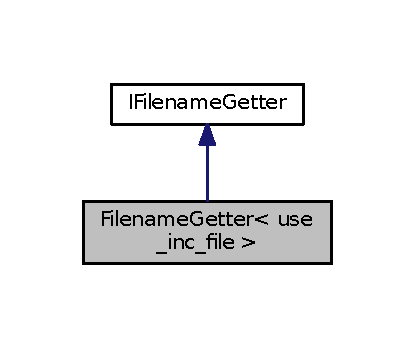
\includegraphics[width=199pt]{struct_filename_getter__inherit__graph}
\end{center}
\end{figure}


Collaboration diagram for Filename\+Getter$<$ use\+\_\+inc\+\_\+file $>$\+:
\nopagebreak
\begin{figure}[H]
\begin{center}
\leavevmode
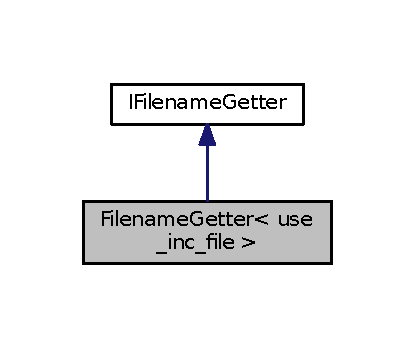
\includegraphics[width=199pt]{struct_filename_getter__coll__graph}
\end{center}
\end{figure}
\subsection*{Public Member Functions}
\begin{DoxyCompactItemize}
\item 
string \hyperlink{struct_filename_getter_a39dfdbff4d78e09117f0e2d98b7044e5}{operator()} (time\+\_\+t time) override
\end{DoxyCompactItemize}
\subsection*{Static Public Member Functions}
\begin{DoxyCompactItemize}
\item 
static string \hyperlink{struct_filename_getter_a3cda4cc7e1fbe66764feef97dc8cfaf6}{time\+To\+String} (time\+\_\+t time)
\end{DoxyCompactItemize}


\subsection{Detailed Description}
\subsubsection*{template$<$bool use\+\_\+inc\+\_\+file = false$>$\\*
struct Filename\+Getter$<$ use\+\_\+inc\+\_\+file $>$}



Definition at line 83 of file observers.\+h.



\subsection{Member Function Documentation}
\index{Filename\+Getter@{Filename\+Getter}!operator()@{operator()}}
\index{operator()@{operator()}!Filename\+Getter@{Filename\+Getter}}
\subsubsection[{\texorpdfstring{operator()(time\+\_\+t time) override}{operator()(time_t time) override}}]{\setlength{\rightskip}{0pt plus 5cm}template$<$bool use\+\_\+inc\+\_\+file = false$>$ string {\bf Filename\+Getter}$<$ use\+\_\+inc\+\_\+file $>$\+::operator() (
\begin{DoxyParamCaption}
\item[{time\+\_\+t}]{time}
\end{DoxyParamCaption}
)\hspace{0.3cm}{\ttfamily [inline]}, {\ttfamily [override]}, {\ttfamily [virtual]}}\hypertarget{struct_filename_getter_a39dfdbff4d78e09117f0e2d98b7044e5}{}\label{struct_filename_getter_a39dfdbff4d78e09117f0e2d98b7044e5}


Implements \hyperlink{struct_i_filename_getter_a91494380c214e12bd0e6bf875c0f5a0d}{I\+Filename\+Getter}.



Definition at line 84 of file observers.\+h.

\index{Filename\+Getter@{Filename\+Getter}!time\+To\+String@{time\+To\+String}}
\index{time\+To\+String@{time\+To\+String}!Filename\+Getter@{Filename\+Getter}}
\subsubsection[{\texorpdfstring{time\+To\+String(time\+\_\+t time)}{timeToString(time_t time)}}]{\setlength{\rightskip}{0pt plus 5cm}template$<$bool use\+\_\+inc\+\_\+file = false$>$ static string {\bf Filename\+Getter}$<$ use\+\_\+inc\+\_\+file $>$\+::time\+To\+String (
\begin{DoxyParamCaption}
\item[{time\+\_\+t}]{time}
\end{DoxyParamCaption}
)\hspace{0.3cm}{\ttfamily [inline]}, {\ttfamily [static]}}\hypertarget{struct_filename_getter_a3cda4cc7e1fbe66764feef97dc8cfaf6}{}\label{struct_filename_getter_a3cda4cc7e1fbe66764feef97dc8cfaf6}


Definition at line 92 of file observers.\+h.



The documentation for this struct was generated from the following file\+:\begin{DoxyCompactItemize}
\item 
\hyperlink{observers_8h}{observers.\+h}\end{DoxyCompactItemize}

\hypertarget{struct_file_output_observer}{}\section{File\+Output\+Observer$<$ use\+\_\+inc\+\_\+file, F\+Name\+Getter $>$ Struct Template Reference}
\label{struct_file_output_observer}\index{File\+Output\+Observer$<$ use\+\_\+inc\+\_\+file, F\+Name\+Getter $>$@{File\+Output\+Observer$<$ use\+\_\+inc\+\_\+file, F\+Name\+Getter $>$}}


{\ttfamily \#include $<$observers.\+h$>$}



Inheritance diagram for File\+Output\+Observer$<$ use\+\_\+inc\+\_\+file, F\+Name\+Getter $>$\+:
\nopagebreak
\begin{figure}[H]
\begin{center}
\leavevmode
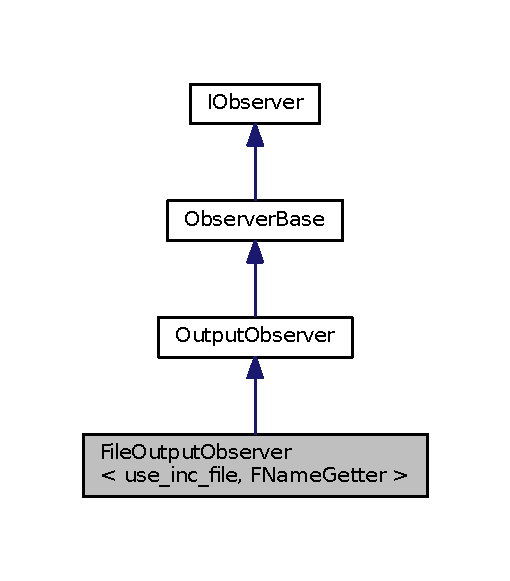
\includegraphics[width=245pt]{struct_file_output_observer__inherit__graph}
\end{center}
\end{figure}


Collaboration diagram for File\+Output\+Observer$<$ use\+\_\+inc\+\_\+file, F\+Name\+Getter $>$\+:
\nopagebreak
\begin{figure}[H]
\begin{center}
\leavevmode
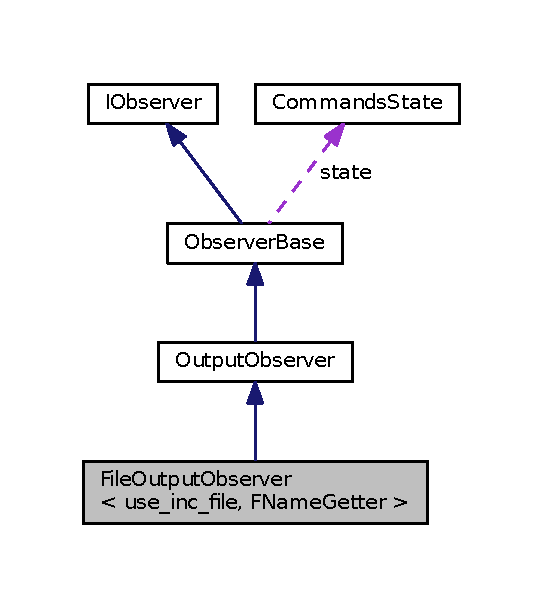
\includegraphics[width=261pt]{struct_file_output_observer__coll__graph}
\end{center}
\end{figure}
\subsection*{Public Member Functions}
\begin{DoxyCompactItemize}
\item 
\hyperlink{struct_file_output_observer_aa4fba0db9135440d1839b78cf3f5d6f2}{File\+Output\+Observer} (\hyperlink{struct_i_observable}{I\+Observable} \&observable, \hyperlink{class_commands_state}{Commands\+State} \&\hyperlink{struct_observer_base_a107ad54040309605fa5fafd481b97f2f}{state})
\item 
std\+::ostream \& \hyperlink{struct_file_output_observer_a29e2740fee9602d0c6ebcb2fe44d2060}{get\+Out\+Stream} () override
\item 
void \hyperlink{struct_file_output_observer_a818d1d56e2495ecfa79a50297a0639ce}{out\+Bulk} () override
\item 
\hyperlink{struct_file_output_observer_ab1ce3fa7b827c1cc13aa231be7612e72}{$\sim$\+File\+Output\+Observer} ()
\end{DoxyCompactItemize}
\subsection*{Static Public Member Functions}
\begin{DoxyCompactItemize}
\item 
static string \hyperlink{struct_file_output_observer_a2fa43d18e8535b246ad2167c3dbd7eaa}{gen\+File\+Name} (time\+\_\+t time)
\end{DoxyCompactItemize}
\subsection*{Additional Inherited Members}


\subsection{Detailed Description}
\subsubsection*{template$<$bool use\+\_\+inc\+\_\+file = false, class F\+Name\+Getter = Filename\+Getter$<$use\+\_\+inc\+\_\+file$>$$>$\\*
struct File\+Output\+Observer$<$ use\+\_\+inc\+\_\+file, F\+Name\+Getter $>$}



Definition at line 102 of file observers.\+h.



\subsection{Constructor \& Destructor Documentation}
\index{File\+Output\+Observer@{File\+Output\+Observer}!File\+Output\+Observer@{File\+Output\+Observer}}
\index{File\+Output\+Observer@{File\+Output\+Observer}!File\+Output\+Observer@{File\+Output\+Observer}}
\subsubsection[{\texorpdfstring{File\+Output\+Observer(\+I\+Observable \&observable, Commands\+State \&state)}{FileOutputObserver(IObservable &observable, CommandsState &state)}}]{\setlength{\rightskip}{0pt plus 5cm}template$<$bool use\+\_\+inc\+\_\+file = false, class F\+Name\+Getter  = Filename\+Getter$<$use\+\_\+inc\+\_\+file$>$$>$ {\bf File\+Output\+Observer}$<$ use\+\_\+inc\+\_\+file, F\+Name\+Getter $>$\+::{\bf File\+Output\+Observer} (
\begin{DoxyParamCaption}
\item[{{\bf I\+Observable} \&}]{observable, }
\item[{{\bf Commands\+State} \&}]{state}
\end{DoxyParamCaption}
)\hspace{0.3cm}{\ttfamily [inline]}}\hypertarget{struct_file_output_observer_aa4fba0db9135440d1839b78cf3f5d6f2}{}\label{struct_file_output_observer_aa4fba0db9135440d1839b78cf3f5d6f2}


Definition at line 103 of file observers.\+h.

\index{File\+Output\+Observer@{File\+Output\+Observer}!````~File\+Output\+Observer@{$\sim$\+File\+Output\+Observer}}
\index{````~File\+Output\+Observer@{$\sim$\+File\+Output\+Observer}!File\+Output\+Observer@{File\+Output\+Observer}}
\subsubsection[{\texorpdfstring{$\sim$\+File\+Output\+Observer()}{~FileOutputObserver()}}]{\setlength{\rightskip}{0pt plus 5cm}template$<$bool use\+\_\+inc\+\_\+file = false, class F\+Name\+Getter  = Filename\+Getter$<$use\+\_\+inc\+\_\+file$>$$>$ {\bf File\+Output\+Observer}$<$ use\+\_\+inc\+\_\+file, F\+Name\+Getter $>$\+::$\sim${\bf File\+Output\+Observer} (
\begin{DoxyParamCaption}
{}
\end{DoxyParamCaption}
)\hspace{0.3cm}{\ttfamily [inline]}}\hypertarget{struct_file_output_observer_ab1ce3fa7b827c1cc13aa231be7612e72}{}\label{struct_file_output_observer_ab1ce3fa7b827c1cc13aa231be7612e72}


Definition at line 120 of file observers.\+h.



\subsection{Member Function Documentation}
\index{File\+Output\+Observer@{File\+Output\+Observer}!gen\+File\+Name@{gen\+File\+Name}}
\index{gen\+File\+Name@{gen\+File\+Name}!File\+Output\+Observer@{File\+Output\+Observer}}
\subsubsection[{\texorpdfstring{gen\+File\+Name(time\+\_\+t time)}{genFileName(time_t time)}}]{\setlength{\rightskip}{0pt plus 5cm}template$<$bool use\+\_\+inc\+\_\+file = false, class F\+Name\+Getter  = Filename\+Getter$<$use\+\_\+inc\+\_\+file$>$$>$ static string {\bf File\+Output\+Observer}$<$ use\+\_\+inc\+\_\+file, F\+Name\+Getter $>$\+::gen\+File\+Name (
\begin{DoxyParamCaption}
\item[{time\+\_\+t}]{time}
\end{DoxyParamCaption}
)\hspace{0.3cm}{\ttfamily [inline]}, {\ttfamily [static]}}\hypertarget{struct_file_output_observer_a2fa43d18e8535b246ad2167c3dbd7eaa}{}\label{struct_file_output_observer_a2fa43d18e8535b246ad2167c3dbd7eaa}


Definition at line 137 of file observers.\+h.

\index{File\+Output\+Observer@{File\+Output\+Observer}!get\+Out\+Stream@{get\+Out\+Stream}}
\index{get\+Out\+Stream@{get\+Out\+Stream}!File\+Output\+Observer@{File\+Output\+Observer}}
\subsubsection[{\texorpdfstring{get\+Out\+Stream() override}{getOutStream() override}}]{\setlength{\rightskip}{0pt plus 5cm}template$<$bool use\+\_\+inc\+\_\+file = false, class F\+Name\+Getter  = Filename\+Getter$<$use\+\_\+inc\+\_\+file$>$$>$ std\+::ostream\& {\bf File\+Output\+Observer}$<$ use\+\_\+inc\+\_\+file, F\+Name\+Getter $>$\+::get\+Out\+Stream (
\begin{DoxyParamCaption}
{}
\end{DoxyParamCaption}
)\hspace{0.3cm}{\ttfamily [inline]}, {\ttfamily [override]}, {\ttfamily [virtual]}}\hypertarget{struct_file_output_observer_a29e2740fee9602d0c6ebcb2fe44d2060}{}\label{struct_file_output_observer_a29e2740fee9602d0c6ebcb2fe44d2060}


Reimplemented from \hyperlink{struct_output_observer_a6a89f9b1dbe4781dd3246f751b73756e}{Output\+Observer}.



Definition at line 105 of file observers.\+h.

\index{File\+Output\+Observer@{File\+Output\+Observer}!out\+Bulk@{out\+Bulk}}
\index{out\+Bulk@{out\+Bulk}!File\+Output\+Observer@{File\+Output\+Observer}}
\subsubsection[{\texorpdfstring{out\+Bulk() override}{outBulk() override}}]{\setlength{\rightskip}{0pt plus 5cm}template$<$bool use\+\_\+inc\+\_\+file = false, class F\+Name\+Getter  = Filename\+Getter$<$use\+\_\+inc\+\_\+file$>$$>$ void {\bf File\+Output\+Observer}$<$ use\+\_\+inc\+\_\+file, F\+Name\+Getter $>$\+::out\+Bulk (
\begin{DoxyParamCaption}
{}
\end{DoxyParamCaption}
)\hspace{0.3cm}{\ttfamily [inline]}, {\ttfamily [override]}, {\ttfamily [virtual]}}\hypertarget{struct_file_output_observer_a818d1d56e2495ecfa79a50297a0639ce}{}\label{struct_file_output_observer_a818d1d56e2495ecfa79a50297a0639ce}


Implements \hyperlink{struct_observer_base_acf405ad8b991810572d0c2425f782b36}{Observer\+Base}.



Definition at line 110 of file observers.\+h.



Here is the call graph for this function\+:
\nopagebreak
\begin{figure}[H]
\begin{center}
\leavevmode
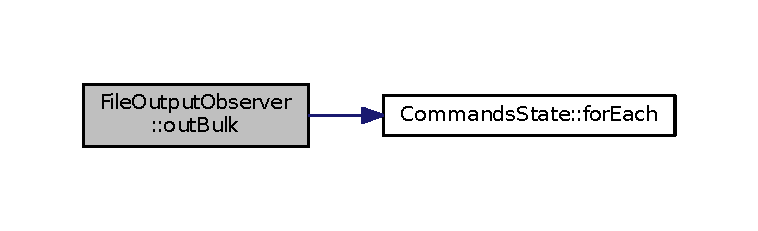
\includegraphics[width=350pt]{struct_file_output_observer_a818d1d56e2495ecfa79a50297a0639ce_cgraph}
\end{center}
\end{figure}




The documentation for this struct was generated from the following file\+:\begin{DoxyCompactItemize}
\item 
\hyperlink{observers_8h}{observers.\+h}\end{DoxyCompactItemize}

\hypertarget{struct_i_command}{}\section{I\+Command$<$ T $>$ Struct Template Reference}
\label{struct_i_command}\index{I\+Command$<$ T $>$@{I\+Command$<$ T $>$}}


{\ttfamily \#include $<$interface.\+h$>$}

\subsection*{Public Member Functions}
\begin{DoxyCompactItemize}
\item 
virtual void \hyperlink{struct_i_command_aa00e7af6e23959c4ffef6d990a0750b2}{exec} (\mbox{[}\mbox{[}maybe\+\_\+unused\mbox{]}\mbox{]} const T \&data=T\{\})=0
\item 
virtual \hyperlink{struct_i_command_a0efde7ae0dd24b4701357a58db9483cd}{$\sim$\+I\+Command} ()
\end{DoxyCompactItemize}


\subsection{Detailed Description}
\subsubsection*{template$<$typename T$>$\\*
struct I\+Command$<$ T $>$}



Definition at line 26 of file interface.\+h.



\subsection{Constructor \& Destructor Documentation}
\index{I\+Command@{I\+Command}!````~I\+Command@{$\sim$\+I\+Command}}
\index{````~I\+Command@{$\sim$\+I\+Command}!I\+Command@{I\+Command}}
\subsubsection[{\texorpdfstring{$\sim$\+I\+Command()}{~ICommand()}}]{\setlength{\rightskip}{0pt plus 5cm}template$<$typename T$>$ virtual {\bf I\+Command}$<$ T $>$\+::$\sim${\bf I\+Command} (
\begin{DoxyParamCaption}
{}
\end{DoxyParamCaption}
)\hspace{0.3cm}{\ttfamily [inline]}, {\ttfamily [virtual]}}\hypertarget{struct_i_command_a0efde7ae0dd24b4701357a58db9483cd}{}\label{struct_i_command_a0efde7ae0dd24b4701357a58db9483cd}


Definition at line 28 of file interface.\+h.



\subsection{Member Function Documentation}
\index{I\+Command@{I\+Command}!exec@{exec}}
\index{exec@{exec}!I\+Command@{I\+Command}}
\subsubsection[{\texorpdfstring{exec([[maybe\+\_\+unused]] const T \&data=T\lcurly{}\rcurly{})=0}{exec([[maybe_unused]] const T &data=T\{\})=0}}]{\setlength{\rightskip}{0pt plus 5cm}template$<$typename T$>$ virtual void {\bf I\+Command}$<$ T $>$\+::exec (
\begin{DoxyParamCaption}
\item[{\mbox{[}\mbox{[}maybe\+\_\+unused\mbox{]} \mbox{]} const T \&}]{data = {\ttfamily T\{\}}}
\end{DoxyParamCaption}
)\hspace{0.3cm}{\ttfamily [pure virtual]}}\hypertarget{struct_i_command_aa00e7af6e23959c4ffef6d990a0750b2}{}\label{struct_i_command_aa00e7af6e23959c4ffef6d990a0750b2}


Implemented in \hyperlink{class_cmd_eof_a8435f64f04c88623fb29168ebf883e0d}{Cmd\+Eof}, \hyperlink{class_cmd_end_a4c316b96ae2a814838a4c985b8b551ab}{Cmd\+End}, and \hyperlink{class_cmd_start_acf20f86d72982205d1af586b5e09846e}{Cmd\+Start}.



The documentation for this struct was generated from the following file\+:\begin{DoxyCompactItemize}
\item 
\hyperlink{interface_8h}{interface.\+h}\end{DoxyCompactItemize}

\hypertarget{struct_i_filename_getter}{}\section{I\+Filename\+Getter Struct Reference}
\label{struct_i_filename_getter}\index{I\+Filename\+Getter@{I\+Filename\+Getter}}


{\ttfamily \#include $<$interface.\+h$>$}



Inheritance diagram for I\+Filename\+Getter\+:
\nopagebreak
\begin{figure}[H]
\begin{center}
\leavevmode
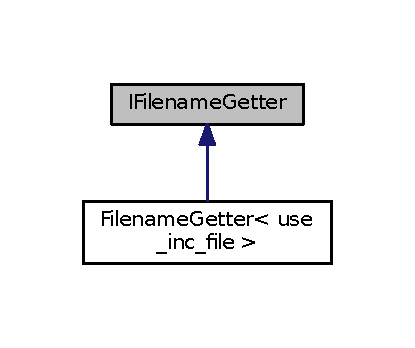
\includegraphics[width=199pt]{struct_i_filename_getter__inherit__graph}
\end{center}
\end{figure}
\subsection*{Public Member Functions}
\begin{DoxyCompactItemize}
\item 
virtual string \hyperlink{struct_i_filename_getter_a91494380c214e12bd0e6bf875c0f5a0d}{operator()} (time\+\_\+t time)=0
\end{DoxyCompactItemize}


\subsection{Detailed Description}


Definition at line 31 of file interface.\+h.



\subsection{Member Function Documentation}
\index{I\+Filename\+Getter@{I\+Filename\+Getter}!operator()@{operator()}}
\index{operator()@{operator()}!I\+Filename\+Getter@{I\+Filename\+Getter}}
\subsubsection[{\texorpdfstring{operator()(time\+\_\+t time)=0}{operator()(time_t time)=0}}]{\setlength{\rightskip}{0pt plus 5cm}virtual string I\+Filename\+Getter\+::operator() (
\begin{DoxyParamCaption}
\item[{time\+\_\+t}]{time}
\end{DoxyParamCaption}
)\hspace{0.3cm}{\ttfamily [pure virtual]}}\hypertarget{struct_i_filename_getter_a91494380c214e12bd0e6bf875c0f5a0d}{}\label{struct_i_filename_getter_a91494380c214e12bd0e6bf875c0f5a0d}


Implemented in \hyperlink{struct_filename_getter_a39dfdbff4d78e09117f0e2d98b7044e5}{Filename\+Getter$<$ use\+\_\+inc\+\_\+file $>$}.



Here is the caller graph for this function\+:
\nopagebreak
\begin{figure}[H]
\begin{center}
\leavevmode
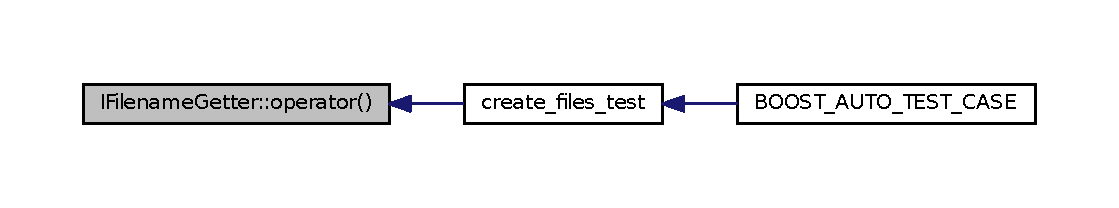
\includegraphics[width=350pt]{struct_i_filename_getter_a91494380c214e12bd0e6bf875c0f5a0d_icgraph}
\end{center}
\end{figure}




The documentation for this struct was generated from the following file\+:\begin{DoxyCompactItemize}
\item 
\hyperlink{interface_8h}{interface.\+h}\end{DoxyCompactItemize}

\hypertarget{struct_i_observable}{}\section{I\+Observable Struct Reference}
\label{struct_i_observable}\index{I\+Observable@{I\+Observable}}


{\ttfamily \#include $<$interface.\+h$>$}



Inheritance diagram for I\+Observable\+:
\nopagebreak
\begin{figure}[H]
\begin{center}
\leavevmode
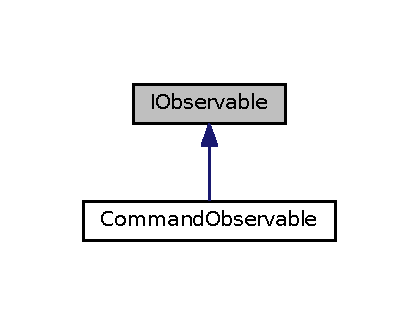
\includegraphics[width=201pt]{struct_i_observable__inherit__graph}
\end{center}
\end{figure}
\subsection*{Public Member Functions}
\begin{DoxyCompactItemize}
\item 
virtual void \hyperlink{struct_i_observable_a20ae9c2f2d4618af71f8eae770f2cadd}{subscribe} (\hyperlink{struct_i_observer}{I\+Observer} $\ast$)=0
\item 
virtual void \hyperlink{struct_i_observable_a639f160d68e626515e6d977f813c3b09}{notify} (\hyperlink{interface_8h_aa299181f275f76f11365a410f7429098}{E\+Command} cmd)=0
\item 
virtual void \hyperlink{struct_i_observable_a457791f8021b05c51ec51193e0392fd3}{notify} (\mbox{[}\mbox{[}maybe\+\_\+unused\mbox{]}\mbox{]} \hyperlink{interface_8h_aa299181f275f76f11365a410f7429098}{E\+Command} cmd, \mbox{[}\mbox{[}maybe\+\_\+unused\mbox{]}\mbox{]} string data)
\item 
virtual \hyperlink{struct_i_observable_ae41e5a178a9ca6a4b83433ffea1d1ce1}{$\sim$\+I\+Observable} ()
\end{DoxyCompactItemize}


\subsection{Detailed Description}


Definition at line 18 of file interface.\+h.



\subsection{Constructor \& Destructor Documentation}
\index{I\+Observable@{I\+Observable}!````~I\+Observable@{$\sim$\+I\+Observable}}
\index{````~I\+Observable@{$\sim$\+I\+Observable}!I\+Observable@{I\+Observable}}
\subsubsection[{\texorpdfstring{$\sim$\+I\+Observable()}{~IObservable()}}]{\setlength{\rightskip}{0pt plus 5cm}virtual I\+Observable\+::$\sim$\+I\+Observable (
\begin{DoxyParamCaption}
{}
\end{DoxyParamCaption}
)\hspace{0.3cm}{\ttfamily [inline]}, {\ttfamily [virtual]}}\hypertarget{struct_i_observable_ae41e5a178a9ca6a4b83433ffea1d1ce1}{}\label{struct_i_observable_ae41e5a178a9ca6a4b83433ffea1d1ce1}


Definition at line 22 of file interface.\+h.



\subsection{Member Function Documentation}
\index{I\+Observable@{I\+Observable}!notify@{notify}}
\index{notify@{notify}!I\+Observable@{I\+Observable}}
\subsubsection[{\texorpdfstring{notify(\+E\+Command cmd)=0}{notify(ECommand cmd)=0}}]{\setlength{\rightskip}{0pt plus 5cm}virtual void I\+Observable\+::notify (
\begin{DoxyParamCaption}
\item[{{\bf E\+Command}}]{cmd}
\end{DoxyParamCaption}
)\hspace{0.3cm}{\ttfamily [pure virtual]}}\hypertarget{struct_i_observable_a639f160d68e626515e6d977f813c3b09}{}\label{struct_i_observable_a639f160d68e626515e6d977f813c3b09}


Implemented in \hyperlink{class_command_observable_a6df1f72513d0964125e6eec93a861335}{Command\+Observable}.



Here is the caller graph for this function\+:
\nopagebreak
\begin{figure}[H]
\begin{center}
\leavevmode
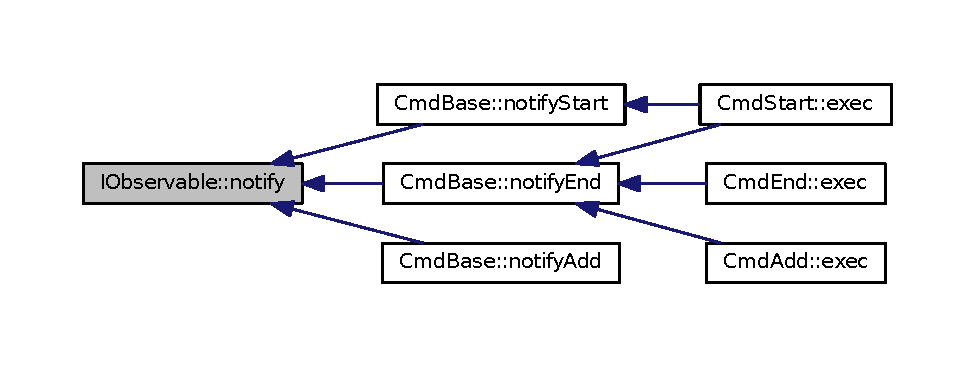
\includegraphics[width=350pt]{struct_i_observable_a639f160d68e626515e6d977f813c3b09_icgraph}
\end{center}
\end{figure}


\index{I\+Observable@{I\+Observable}!notify@{notify}}
\index{notify@{notify}!I\+Observable@{I\+Observable}}
\subsubsection[{\texorpdfstring{notify([[maybe\+\_\+unused]] E\+Command cmd, [[maybe\+\_\+unused]] string data)}{notify([[maybe_unused]] ECommand cmd, [[maybe_unused]] string data)}}]{\setlength{\rightskip}{0pt plus 5cm}virtual void I\+Observable\+::notify (
\begin{DoxyParamCaption}
\item[{\mbox{[}\mbox{[}maybe\+\_\+unused\mbox{]} \mbox{]} {\bf E\+Command}}]{cmd, }
\item[{\mbox{[}\mbox{[}maybe\+\_\+unused\mbox{]} \mbox{]} string}]{data}
\end{DoxyParamCaption}
)\hspace{0.3cm}{\ttfamily [inline]}, {\ttfamily [virtual]}}\hypertarget{struct_i_observable_a457791f8021b05c51ec51193e0392fd3}{}\label{struct_i_observable_a457791f8021b05c51ec51193e0392fd3}


Definition at line 21 of file interface.\+h.

\index{I\+Observable@{I\+Observable}!subscribe@{subscribe}}
\index{subscribe@{subscribe}!I\+Observable@{I\+Observable}}
\subsubsection[{\texorpdfstring{subscribe(\+I\+Observer $\ast$)=0}{subscribe(IObserver *)=0}}]{\setlength{\rightskip}{0pt plus 5cm}virtual void I\+Observable\+::subscribe (
\begin{DoxyParamCaption}
\item[{{\bf I\+Observer} $\ast$}]{}
\end{DoxyParamCaption}
)\hspace{0.3cm}{\ttfamily [pure virtual]}}\hypertarget{struct_i_observable_a20ae9c2f2d4618af71f8eae770f2cadd}{}\label{struct_i_observable_a20ae9c2f2d4618af71f8eae770f2cadd}


Implemented in \hyperlink{class_command_observable_ad8bc68d264feb6c62ba2964e57c7c1ac}{Command\+Observable}.



The documentation for this struct was generated from the following file\+:\begin{DoxyCompactItemize}
\item 
\hyperlink{interface_8h}{interface.\+h}\end{DoxyCompactItemize}

\hypertarget{struct_i_observer}{}\section{I\+Observer Struct Reference}
\label{struct_i_observer}\index{I\+Observer@{I\+Observer}}


{\ttfamily \#include $<$interface.\+h$>$}



Inheritance diagram for I\+Observer\+:
\nopagebreak
\begin{figure}[H]
\begin{center}
\leavevmode
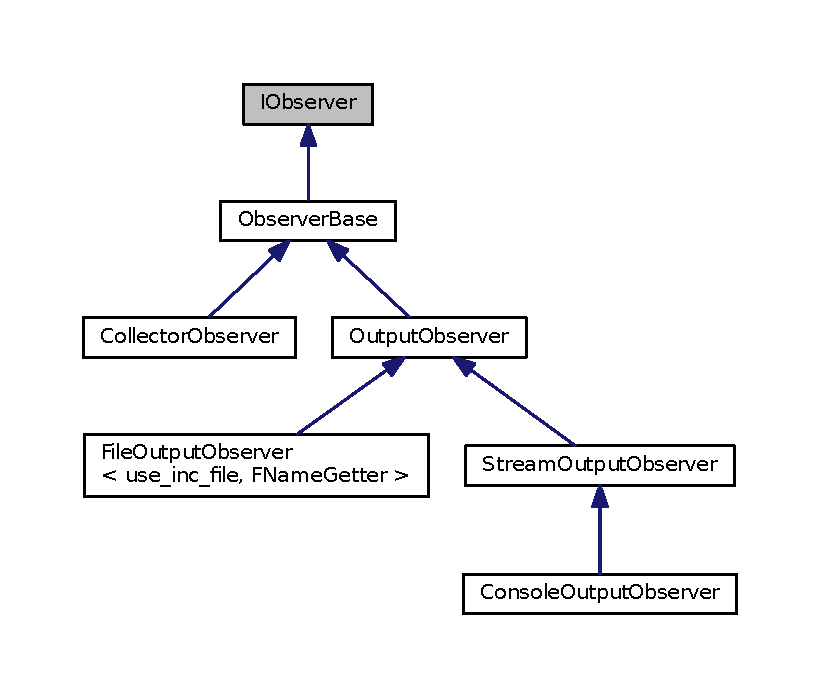
\includegraphics[width=350pt]{struct_i_observer__inherit__graph}
\end{center}
\end{figure}
\subsection*{Public Member Functions}
\begin{DoxyCompactItemize}
\item 
virtual void \hyperlink{struct_i_observer_a8e86c5a6f02b990dc8ee5bb8a546a056}{update} (\hyperlink{interface_8h_aa299181f275f76f11365a410f7429098}{E\+Command} cmd)=0
\item 
virtual void \hyperlink{struct_i_observer_a87304ed05adacf4219c5e4252629ae14}{update} (\hyperlink{interface_8h_aa299181f275f76f11365a410f7429098}{E\+Command} cmd, string data)=0
\item 
virtual \hyperlink{struct_i_observer_afdfe9e2ebd9aa794142968de574daa9a}{$\sim$\+I\+Observer} ()
\end{DoxyCompactItemize}


\subsection{Detailed Description}


Definition at line 12 of file interface.\+h.



\subsection{Constructor \& Destructor Documentation}
\index{I\+Observer@{I\+Observer}!````~I\+Observer@{$\sim$\+I\+Observer}}
\index{````~I\+Observer@{$\sim$\+I\+Observer}!I\+Observer@{I\+Observer}}
\subsubsection[{\texorpdfstring{$\sim$\+I\+Observer()}{~IObserver()}}]{\setlength{\rightskip}{0pt plus 5cm}virtual I\+Observer\+::$\sim$\+I\+Observer (
\begin{DoxyParamCaption}
{}
\end{DoxyParamCaption}
)\hspace{0.3cm}{\ttfamily [inline]}, {\ttfamily [virtual]}}\hypertarget{struct_i_observer_afdfe9e2ebd9aa794142968de574daa9a}{}\label{struct_i_observer_afdfe9e2ebd9aa794142968de574daa9a}


Definition at line 15 of file interface.\+h.



\subsection{Member Function Documentation}
\index{I\+Observer@{I\+Observer}!update@{update}}
\index{update@{update}!I\+Observer@{I\+Observer}}
\subsubsection[{\texorpdfstring{update(\+E\+Command cmd)=0}{update(ECommand cmd)=0}}]{\setlength{\rightskip}{0pt plus 5cm}virtual void I\+Observer\+::update (
\begin{DoxyParamCaption}
\item[{{\bf E\+Command}}]{cmd}
\end{DoxyParamCaption}
)\hspace{0.3cm}{\ttfamily [pure virtual]}}\hypertarget{struct_i_observer_a8e86c5a6f02b990dc8ee5bb8a546a056}{}\label{struct_i_observer_a8e86c5a6f02b990dc8ee5bb8a546a056}


Implemented in \hyperlink{struct_observer_base_ae178c765ecda0166fd784dcb4ebe0a40}{Observer\+Base}.

\index{I\+Observer@{I\+Observer}!update@{update}}
\index{update@{update}!I\+Observer@{I\+Observer}}
\subsubsection[{\texorpdfstring{update(\+E\+Command cmd, string data)=0}{update(ECommand cmd, string data)=0}}]{\setlength{\rightskip}{0pt plus 5cm}virtual void I\+Observer\+::update (
\begin{DoxyParamCaption}
\item[{{\bf E\+Command}}]{cmd, }
\item[{string}]{data}
\end{DoxyParamCaption}
)\hspace{0.3cm}{\ttfamily [pure virtual]}}\hypertarget{struct_i_observer_a87304ed05adacf4219c5e4252629ae14}{}\label{struct_i_observer_a87304ed05adacf4219c5e4252629ae14}


Implemented in \hyperlink{struct_collector_observer_adebc5768f5778ceb3e981362363db247}{Collector\+Observer}.



The documentation for this struct was generated from the following file\+:\begin{DoxyCompactItemize}
\item 
\hyperlink{interface_8h}{interface.\+h}\end{DoxyCompactItemize}

\hypertarget{struct_observer_base}{}\section{Observer\+Base Struct Reference}
\label{struct_observer_base}\index{Observer\+Base@{Observer\+Base}}


{\ttfamily \#include $<$observers.\+h$>$}



Inheritance diagram for Observer\+Base\+:
\nopagebreak
\begin{figure}[H]
\begin{center}
\leavevmode
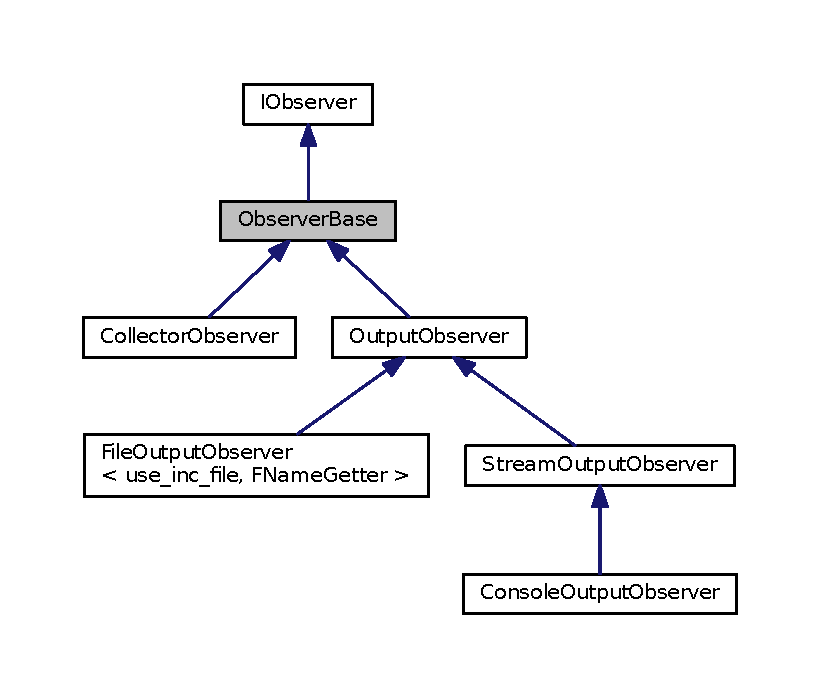
\includegraphics[width=350pt]{struct_observer_base__inherit__graph}
\end{center}
\end{figure}


Collaboration diagram for Observer\+Base\+:
\nopagebreak
\begin{figure}[H]
\begin{center}
\leavevmode
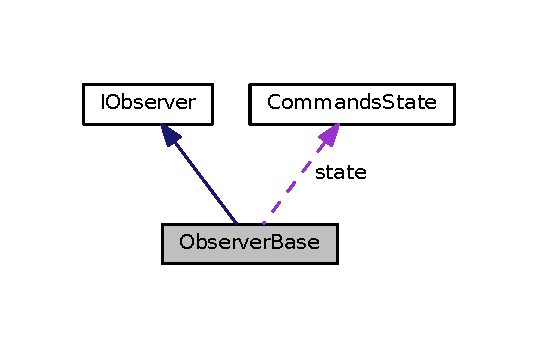
\includegraphics[width=258pt]{struct_observer_base__coll__graph}
\end{center}
\end{figure}
\subsection*{Public Member Functions}
\begin{DoxyCompactItemize}
\item 
\hyperlink{struct_observer_base_ade5a5f743b630b7a3a06c097e7f48aa8}{Observer\+Base} (\hyperlink{struct_i_observable}{I\+Observable} \&observable, \hyperlink{class_commands_state}{Commands\+State} \&\hyperlink{struct_observer_base_a107ad54040309605fa5fafd481b97f2f}{state})
\end{DoxyCompactItemize}
\subsection*{Protected Member Functions}
\begin{DoxyCompactItemize}
\item 
virtual void \hyperlink{struct_observer_base_acf405ad8b991810572d0c2425f782b36}{out\+Bulk} ()=0
\item 
void \hyperlink{struct_observer_base_ae178c765ecda0166fd784dcb4ebe0a40}{update} (\hyperlink{interface_8h_aa299181f275f76f11365a410f7429098}{E\+Command} cmd) override
\item 
void \hyperlink{struct_observer_base_adeede05d3ddea8da1148cdce92f07787}{update} (\hyperlink{interface_8h_aa299181f275f76f11365a410f7429098}{E\+Command} cmd, string data) override
\end{DoxyCompactItemize}
\subsection*{Protected Attributes}
\begin{DoxyCompactItemize}
\item 
\hyperlink{class_commands_state}{Commands\+State} \& \hyperlink{struct_observer_base_a107ad54040309605fa5fafd481b97f2f}{state}
\end{DoxyCompactItemize}


\subsection{Detailed Description}


Definition at line 13 of file observers.\+h.



\subsection{Constructor \& Destructor Documentation}
\index{Observer\+Base@{Observer\+Base}!Observer\+Base@{Observer\+Base}}
\index{Observer\+Base@{Observer\+Base}!Observer\+Base@{Observer\+Base}}
\subsubsection[{\texorpdfstring{Observer\+Base(\+I\+Observable \&observable, Commands\+State \&state)}{ObserverBase(IObservable &observable, CommandsState &state)}}]{\setlength{\rightskip}{0pt plus 5cm}Observer\+Base\+::\+Observer\+Base (
\begin{DoxyParamCaption}
\item[{{\bf I\+Observable} \&}]{observable, }
\item[{{\bf Commands\+State} \&}]{state}
\end{DoxyParamCaption}
)\hspace{0.3cm}{\ttfamily [inline]}}\hypertarget{struct_observer_base_ade5a5f743b630b7a3a06c097e7f48aa8}{}\label{struct_observer_base_ade5a5f743b630b7a3a06c097e7f48aa8}


Definition at line 14 of file observers.\+h.



\subsection{Member Function Documentation}
\index{Observer\+Base@{Observer\+Base}!out\+Bulk@{out\+Bulk}}
\index{out\+Bulk@{out\+Bulk}!Observer\+Base@{Observer\+Base}}
\subsubsection[{\texorpdfstring{out\+Bulk()=0}{outBulk()=0}}]{\setlength{\rightskip}{0pt plus 5cm}virtual void Observer\+Base\+::out\+Bulk (
\begin{DoxyParamCaption}
{}
\end{DoxyParamCaption}
)\hspace{0.3cm}{\ttfamily [protected]}, {\ttfamily [pure virtual]}}\hypertarget{struct_observer_base_acf405ad8b991810572d0c2425f782b36}{}\label{struct_observer_base_acf405ad8b991810572d0c2425f782b36}


Implemented in \hyperlink{struct_file_output_observer_a818d1d56e2495ecfa79a50297a0639ce}{File\+Output\+Observer$<$ use\+\_\+inc\+\_\+file, F\+Name\+Getter $>$}, and \hyperlink{struct_stream_output_observer_a10b38ed3f4f8ef4ffa710830c4229d35}{Stream\+Output\+Observer}.



Here is the caller graph for this function\+:
\nopagebreak
\begin{figure}[H]
\begin{center}
\leavevmode
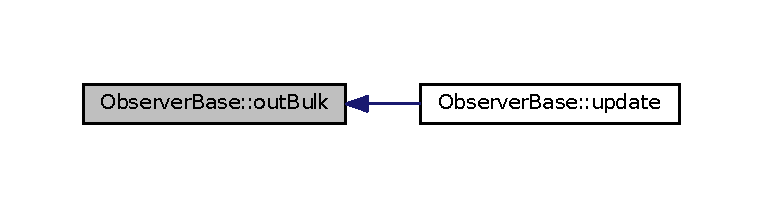
\includegraphics[width=350pt]{struct_observer_base_acf405ad8b991810572d0c2425f782b36_icgraph}
\end{center}
\end{figure}


\index{Observer\+Base@{Observer\+Base}!update@{update}}
\index{update@{update}!Observer\+Base@{Observer\+Base}}
\subsubsection[{\texorpdfstring{update(\+E\+Command cmd) override}{update(ECommand cmd) override}}]{\setlength{\rightskip}{0pt plus 5cm}void Observer\+Base\+::update (
\begin{DoxyParamCaption}
\item[{{\bf E\+Command}}]{cmd}
\end{DoxyParamCaption}
)\hspace{0.3cm}{\ttfamily [inline]}, {\ttfamily [override]}, {\ttfamily [protected]}, {\ttfamily [virtual]}}\hypertarget{struct_observer_base_ae178c765ecda0166fd784dcb4ebe0a40}{}\label{struct_observer_base_ae178c765ecda0166fd784dcb4ebe0a40}


Implements \hyperlink{struct_i_observer_a8e86c5a6f02b990dc8ee5bb8a546a056}{I\+Observer}.



Definition at line 22 of file observers.\+h.



Here is the call graph for this function\+:
\nopagebreak
\begin{figure}[H]
\begin{center}
\leavevmode
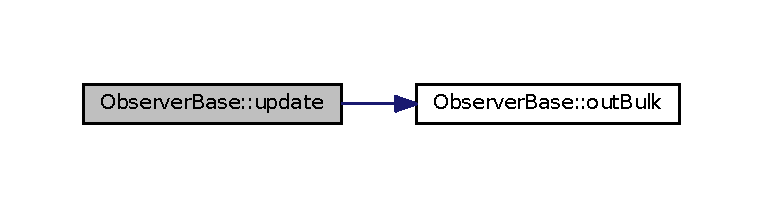
\includegraphics[width=350pt]{struct_observer_base_ae178c765ecda0166fd784dcb4ebe0a40_cgraph}
\end{center}
\end{figure}


\index{Observer\+Base@{Observer\+Base}!update@{update}}
\index{update@{update}!Observer\+Base@{Observer\+Base}}
\subsubsection[{\texorpdfstring{update(\+E\+Command cmd, string data) override}{update(ECommand cmd, string data) override}}]{\setlength{\rightskip}{0pt plus 5cm}void Observer\+Base\+::update (
\begin{DoxyParamCaption}
\item[{{\bf E\+Command}}]{cmd, }
\item[{string}]{data}
\end{DoxyParamCaption}
)\hspace{0.3cm}{\ttfamily [inline]}, {\ttfamily [override]}, {\ttfamily [protected]}, {\ttfamily [virtual]}}\hypertarget{struct_observer_base_adeede05d3ddea8da1148cdce92f07787}{}\label{struct_observer_base_adeede05d3ddea8da1148cdce92f07787}


Implements \hyperlink{struct_i_observer_a87304ed05adacf4219c5e4252629ae14}{I\+Observer}.



Reimplemented in \hyperlink{struct_collector_observer_adebc5768f5778ceb3e981362363db247}{Collector\+Observer}.



Definition at line 31 of file observers.\+h.



\subsection{Member Data Documentation}
\index{Observer\+Base@{Observer\+Base}!state@{state}}
\index{state@{state}!Observer\+Base@{Observer\+Base}}
\subsubsection[{\texorpdfstring{state}{state}}]{\setlength{\rightskip}{0pt plus 5cm}{\bf Commands\+State}\& Observer\+Base\+::state\hspace{0.3cm}{\ttfamily [protected]}}\hypertarget{struct_observer_base_a107ad54040309605fa5fafd481b97f2f}{}\label{struct_observer_base_a107ad54040309605fa5fafd481b97f2f}


Definition at line 18 of file observers.\+h.



The documentation for this struct was generated from the following file\+:\begin{DoxyCompactItemize}
\item 
\hyperlink{observers_8h}{observers.\+h}\end{DoxyCompactItemize}

\hypertarget{struct_output_observer}{}\section{Output\+Observer Struct Reference}
\label{struct_output_observer}\index{Output\+Observer@{Output\+Observer}}


{\ttfamily \#include $<$observers.\+h$>$}



Inheritance diagram for Output\+Observer\+:
\nopagebreak
\begin{figure}[H]
\begin{center}
\leavevmode
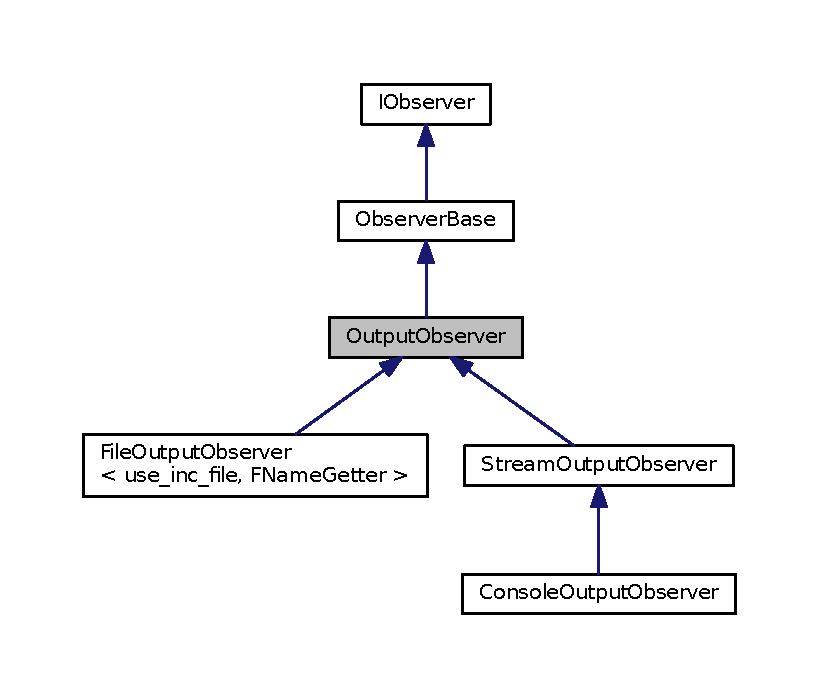
\includegraphics[width=350pt]{struct_output_observer__inherit__graph}
\end{center}
\end{figure}


Collaboration diagram for Output\+Observer\+:
\nopagebreak
\begin{figure}[H]
\begin{center}
\leavevmode
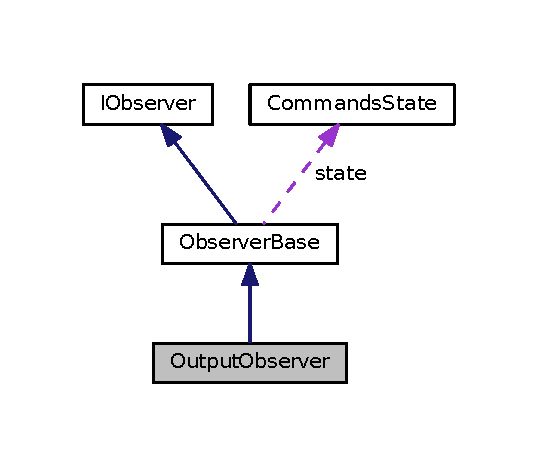
\includegraphics[width=258pt]{struct_output_observer__coll__graph}
\end{center}
\end{figure}
\subsection*{Public Member Functions}
\begin{DoxyCompactItemize}
\item 
\hyperlink{struct_output_observer_a4052d1e6dc1982c34d2d16096e07907d}{Output\+Observer} (\hyperlink{struct_i_observable}{I\+Observable} \&observable, \hyperlink{class_commands_state}{Commands\+State} \&\hyperlink{struct_observer_base_a107ad54040309605fa5fafd481b97f2f}{state})
\item 
virtual void \hyperlink{struct_output_observer_ad570c99b8a3d989e79d3e9da84cf1db3}{set\+Out\+Stream} (std\+::ostream $\ast$\hyperlink{struct_output_observer_a64538320bd2f95c23e7d5d5315aeae7d}{out})
\item 
virtual std\+::ostream \& \hyperlink{struct_output_observer_a6a89f9b1dbe4781dd3246f751b73756e}{get\+Out\+Stream} ()
\end{DoxyCompactItemize}
\subsection*{Protected Attributes}
\begin{DoxyCompactItemize}
\item 
std\+::ostream $\ast$ \hyperlink{struct_output_observer_a64538320bd2f95c23e7d5d5315aeae7d}{out}
\end{DoxyCompactItemize}
\subsection*{Additional Inherited Members}


\subsection{Detailed Description}


Definition at line 47 of file observers.\+h.



\subsection{Constructor \& Destructor Documentation}
\index{Output\+Observer@{Output\+Observer}!Output\+Observer@{Output\+Observer}}
\index{Output\+Observer@{Output\+Observer}!Output\+Observer@{Output\+Observer}}
\subsubsection[{\texorpdfstring{Output\+Observer(\+I\+Observable \&observable, Commands\+State \&state)}{OutputObserver(IObservable &observable, CommandsState &state)}}]{\setlength{\rightskip}{0pt plus 5cm}Output\+Observer\+::\+Output\+Observer (
\begin{DoxyParamCaption}
\item[{{\bf I\+Observable} \&}]{observable, }
\item[{{\bf Commands\+State} \&}]{state}
\end{DoxyParamCaption}
)\hspace{0.3cm}{\ttfamily [inline]}}\hypertarget{struct_output_observer_a4052d1e6dc1982c34d2d16096e07907d}{}\label{struct_output_observer_a4052d1e6dc1982c34d2d16096e07907d}


Definition at line 48 of file observers.\+h.



\subsection{Member Function Documentation}
\index{Output\+Observer@{Output\+Observer}!get\+Out\+Stream@{get\+Out\+Stream}}
\index{get\+Out\+Stream@{get\+Out\+Stream}!Output\+Observer@{Output\+Observer}}
\subsubsection[{\texorpdfstring{get\+Out\+Stream()}{getOutStream()}}]{\setlength{\rightskip}{0pt plus 5cm}virtual std\+::ostream\& Output\+Observer\+::get\+Out\+Stream (
\begin{DoxyParamCaption}
{}
\end{DoxyParamCaption}
)\hspace{0.3cm}{\ttfamily [inline]}, {\ttfamily [virtual]}}\hypertarget{struct_output_observer_a6a89f9b1dbe4781dd3246f751b73756e}{}\label{struct_output_observer_a6a89f9b1dbe4781dd3246f751b73756e}


Reimplemented in \hyperlink{struct_file_output_observer_a29e2740fee9602d0c6ebcb2fe44d2060}{File\+Output\+Observer$<$ use\+\_\+inc\+\_\+file, F\+Name\+Getter $>$}.



Definition at line 52 of file observers.\+h.

\index{Output\+Observer@{Output\+Observer}!set\+Out\+Stream@{set\+Out\+Stream}}
\index{set\+Out\+Stream@{set\+Out\+Stream}!Output\+Observer@{Output\+Observer}}
\subsubsection[{\texorpdfstring{set\+Out\+Stream(std\+::ostream $\ast$out)}{setOutStream(std::ostream *out)}}]{\setlength{\rightskip}{0pt plus 5cm}virtual void Output\+Observer\+::set\+Out\+Stream (
\begin{DoxyParamCaption}
\item[{std\+::ostream $\ast$}]{out}
\end{DoxyParamCaption}
)\hspace{0.3cm}{\ttfamily [inline]}, {\ttfamily [virtual]}}\hypertarget{struct_output_observer_ad570c99b8a3d989e79d3e9da84cf1db3}{}\label{struct_output_observer_ad570c99b8a3d989e79d3e9da84cf1db3}


Definition at line 49 of file observers.\+h.



\subsection{Member Data Documentation}
\index{Output\+Observer@{Output\+Observer}!out@{out}}
\index{out@{out}!Output\+Observer@{Output\+Observer}}
\subsubsection[{\texorpdfstring{out}{out}}]{\setlength{\rightskip}{0pt plus 5cm}std\+::ostream$\ast$ Output\+Observer\+::out\hspace{0.3cm}{\ttfamily [protected]}}\hypertarget{struct_output_observer_a64538320bd2f95c23e7d5d5315aeae7d}{}\label{struct_output_observer_a64538320bd2f95c23e7d5d5315aeae7d}


Definition at line 56 of file observers.\+h.



The documentation for this struct was generated from the following file\+:\begin{DoxyCompactItemize}
\item 
\hyperlink{observers_8h}{observers.\+h}\end{DoxyCompactItemize}

\hypertarget{class_processing}{}\section{Processing Class Reference}
\label{class_processing}\index{Processing@{Processing}}
\subsection*{Public Member Functions}
\begin{DoxyCompactItemize}
\item 
\hyperlink{class_processing_a69199047ad45cb4dcb02b2d281b44264}{Processing} (int limit)
\item 
{\footnotesize template$<$typename In\+Stream $>$ }\\void \hyperlink{class_processing_a69a7389c439fdec2afe57e6e59d5287c}{process\+Input} (In\+Stream \&in)
\end{DoxyCompactItemize}


\subsection{Detailed Description}


Definition at line 25 of file main.\+cpp.



\subsection{Constructor \& Destructor Documentation}
\index{Processing@{Processing}!Processing@{Processing}}
\index{Processing@{Processing}!Processing@{Processing}}
\subsubsection[{\texorpdfstring{Processing(int limit)}{Processing(int limit)}}]{\setlength{\rightskip}{0pt plus 5cm}Processing\+::\+Processing (
\begin{DoxyParamCaption}
\item[{int}]{limit}
\end{DoxyParamCaption}
)\hspace{0.3cm}{\ttfamily [inline]}}\hypertarget{class_processing_a69199047ad45cb4dcb02b2d281b44264}{}\label{class_processing_a69199047ad45cb4dcb02b2d281b44264}


Definition at line 28 of file main.\+cpp.



\subsection{Member Function Documentation}
\index{Processing@{Processing}!process\+Input@{process\+Input}}
\index{process\+Input@{process\+Input}!Processing@{Processing}}
\subsubsection[{\texorpdfstring{process\+Input(\+In\+Stream \&in)}{processInput(InStream &in)}}]{\setlength{\rightskip}{0pt plus 5cm}template$<$typename In\+Stream $>$ void Processing\+::process\+Input (
\begin{DoxyParamCaption}
\item[{In\+Stream \&}]{in}
\end{DoxyParamCaption}
)\hspace{0.3cm}{\ttfamily [inline]}}\hypertarget{class_processing_a69a7389c439fdec2afe57e6e59d5287c}{}\label{class_processing_a69a7389c439fdec2afe57e6e59d5287c}


Definition at line 31 of file main.\+cpp.



Here is the call graph for this function\+:
\nopagebreak
\begin{figure}[H]
\begin{center}
\leavevmode
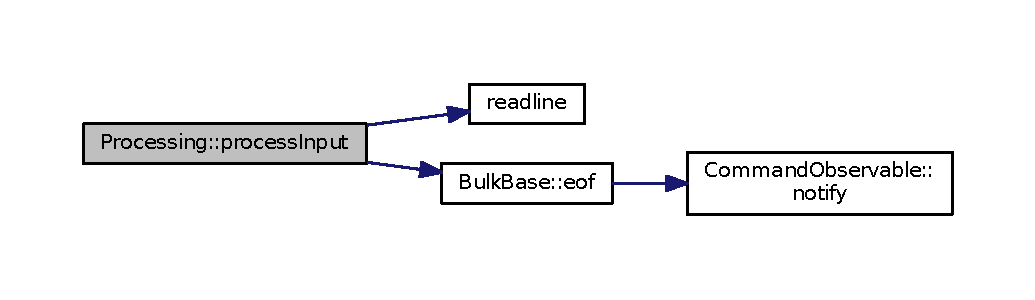
\includegraphics[width=350pt]{class_processing_a69a7389c439fdec2afe57e6e59d5287c_cgraph}
\end{center}
\end{figure}




The documentation for this class was generated from the following file\+:\begin{DoxyCompactItemize}
\item 
\hyperlink{main_8cpp}{main.\+cpp}\end{DoxyCompactItemize}

\hypertarget{struct_stream_output_observer}{}\section{Stream\+Output\+Observer Struct Reference}
\label{struct_stream_output_observer}\index{Stream\+Output\+Observer@{Stream\+Output\+Observer}}


{\ttfamily \#include $<$observers.\+h$>$}



Inheritance diagram for Stream\+Output\+Observer\+:
\nopagebreak
\begin{figure}[H]
\begin{center}
\leavevmode
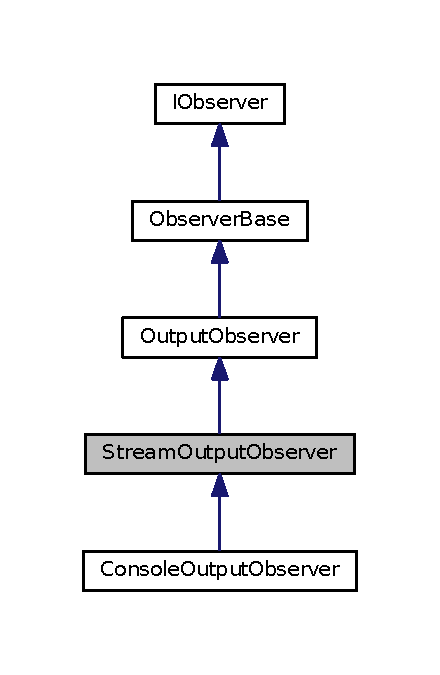
\includegraphics[width=211pt]{struct_stream_output_observer__inherit__graph}
\end{center}
\end{figure}


Collaboration diagram for Stream\+Output\+Observer\+:
\nopagebreak
\begin{figure}[H]
\begin{center}
\leavevmode
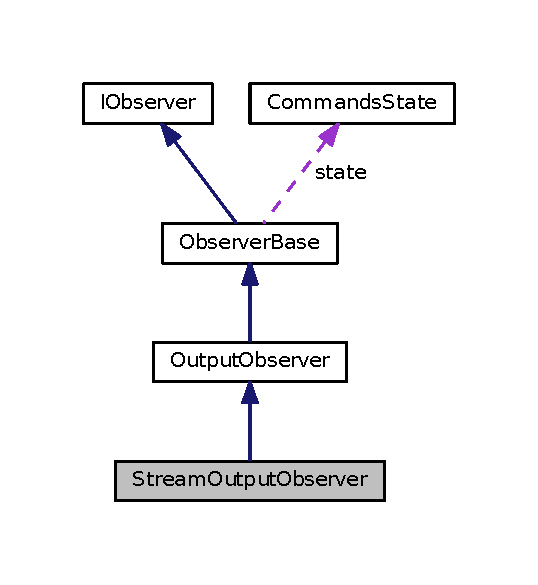
\includegraphics[width=258pt]{struct_stream_output_observer__coll__graph}
\end{center}
\end{figure}
\subsection*{Public Member Functions}
\begin{DoxyCompactItemize}
\item 
\hyperlink{struct_stream_output_observer_a16d3924d3b60bf4e8f12ba372ec86df0}{Stream\+Output\+Observer} (\hyperlink{struct_i_observable}{I\+Observable} \&observable, \hyperlink{class_commands_state}{Commands\+State} \&\hyperlink{struct_observer_base_a107ad54040309605fa5fafd481b97f2f}{state})
\item 
void \hyperlink{struct_stream_output_observer_a10b38ed3f4f8ef4ffa710830c4229d35}{out\+Bulk} () override
\end{DoxyCompactItemize}
\subsection*{Additional Inherited Members}


\subsection{Detailed Description}


Definition at line 59 of file observers.\+h.



\subsection{Constructor \& Destructor Documentation}
\index{Stream\+Output\+Observer@{Stream\+Output\+Observer}!Stream\+Output\+Observer@{Stream\+Output\+Observer}}
\index{Stream\+Output\+Observer@{Stream\+Output\+Observer}!Stream\+Output\+Observer@{Stream\+Output\+Observer}}
\subsubsection[{\texorpdfstring{Stream\+Output\+Observer(\+I\+Observable \&observable, Commands\+State \&state)}{StreamOutputObserver(IObservable &observable, CommandsState &state)}}]{\setlength{\rightskip}{0pt plus 5cm}Stream\+Output\+Observer\+::\+Stream\+Output\+Observer (
\begin{DoxyParamCaption}
\item[{{\bf I\+Observable} \&}]{observable, }
\item[{{\bf Commands\+State} \&}]{state}
\end{DoxyParamCaption}
)\hspace{0.3cm}{\ttfamily [inline]}}\hypertarget{struct_stream_output_observer_a16d3924d3b60bf4e8f12ba372ec86df0}{}\label{struct_stream_output_observer_a16d3924d3b60bf4e8f12ba372ec86df0}


Definition at line 60 of file observers.\+h.



\subsection{Member Function Documentation}
\index{Stream\+Output\+Observer@{Stream\+Output\+Observer}!out\+Bulk@{out\+Bulk}}
\index{out\+Bulk@{out\+Bulk}!Stream\+Output\+Observer@{Stream\+Output\+Observer}}
\subsubsection[{\texorpdfstring{out\+Bulk() override}{outBulk() override}}]{\setlength{\rightskip}{0pt plus 5cm}void Stream\+Output\+Observer\+::out\+Bulk (
\begin{DoxyParamCaption}
{}
\end{DoxyParamCaption}
)\hspace{0.3cm}{\ttfamily [inline]}, {\ttfamily [override]}, {\ttfamily [virtual]}}\hypertarget{struct_stream_output_observer_a10b38ed3f4f8ef4ffa710830c4229d35}{}\label{struct_stream_output_observer_a10b38ed3f4f8ef4ffa710830c4229d35}


Implements \hyperlink{struct_observer_base_acf405ad8b991810572d0c2425f782b36}{Observer\+Base}.



Definition at line 61 of file observers.\+h.



Here is the call graph for this function\+:
\nopagebreak
\begin{figure}[H]
\begin{center}
\leavevmode
\includegraphics[width=350pt]{struct_stream_output_observer_a10b38ed3f4f8ef4ffa710830c4229d35_cgraph}
\end{center}
\end{figure}




The documentation for this struct was generated from the following file\+:\begin{DoxyCompactItemize}
\item 
\hyperlink{observers_8h}{observers.\+h}\end{DoxyCompactItemize}

\chapter{File Documentation}
\hypertarget{bulk_8h}{}\section{bulk.\+h File Reference}
\label{bulk_8h}\index{bulk.\+h@{bulk.\+h}}
{\ttfamily \#include \char`\"{}share.\+h\char`\"{}}\\*
{\ttfamily \#include $<$string$>$}\\*
{\ttfamily \#include $<$vector$>$}\\*
{\ttfamily \#include \char`\"{}interface.\+h\char`\"{}}\\*
{\ttfamily \#include \char`\"{}observers.\+h\char`\"{}}\\*
{\ttfamily \#include \char`\"{}commands.\+h\char`\"{}}\\*
{\ttfamily \#include $<$iostream$>$}\\*
Include dependency graph for bulk.\+h\+:
\nopagebreak
\begin{figure}[H]
\begin{center}
\leavevmode
\includegraphics[width=350pt]{bulk_8h__incl}
\end{center}
\end{figure}
This graph shows which files directly or indirectly include this file\+:
\nopagebreak
\begin{figure}[H]
\begin{center}
\leavevmode
\includegraphics[width=220pt]{bulk_8h__dep__incl}
\end{center}
\end{figure}
\subsection*{Classes}
\begin{DoxyCompactItemize}
\item 
class \hyperlink{class_bulk_base}{Bulk\+Base$<$ Out\+Observers $>$}
\end{DoxyCompactItemize}
\subsection*{Typedefs}
\begin{DoxyCompactItemize}
\item 
using \hyperlink{bulk_8h_a053512dbc7e1702b7968b31b976b23cd}{Bulk} = \hyperlink{class_bulk_base}{Bulk\+Base}$<$ \hyperlink{struct_console_output_observer}{Console\+Output\+Observer}, \hyperlink{struct_file_output_observer}{File\+Output\+Observer}$<$$>$$>$
\end{DoxyCompactItemize}


\subsection{Typedef Documentation}
\index{bulk.\+h@{bulk.\+h}!Bulk@{Bulk}}
\index{Bulk@{Bulk}!bulk.\+h@{bulk.\+h}}
\subsubsection[{\texorpdfstring{Bulk}{Bulk}}]{\setlength{\rightskip}{0pt plus 5cm}using {\bf Bulk} =  {\bf Bulk\+Base}$<$ {\bf Console\+Output\+Observer}, {\bf File\+Output\+Observer}$<$$>$$>$}\hypertarget{bulk_8h_a053512dbc7e1702b7968b31b976b23cd}{}\label{bulk_8h_a053512dbc7e1702b7968b31b976b23cd}


Definition at line 56 of file bulk.\+h.


\hypertarget{commands_8h}{}\section{commands.\+h File Reference}
\label{commands_8h}\index{commands.\+h@{commands.\+h}}
{\ttfamily \#include $<$map$>$}\\*
{\ttfamily \#include \char`\"{}interface.\+h\char`\"{}}\\*
{\ttfamily \#include \char`\"{}state.\+h\char`\"{}}\\*
Include dependency graph for commands.\+h\+:
\nopagebreak
\begin{figure}[H]
\begin{center}
\leavevmode
\includegraphics[width=350pt]{commands_8h__incl}
\end{center}
\end{figure}
This graph shows which files directly or indirectly include this file\+:
\nopagebreak
\begin{figure}[H]
\begin{center}
\leavevmode
\includegraphics[width=220pt]{commands_8h__dep__incl}
\end{center}
\end{figure}
\subsection*{Classes}
\begin{DoxyCompactItemize}
\item 
class \hyperlink{class_cmd_base}{Cmd\+Base}
\item 
class \hyperlink{class_cmd_start}{Cmd\+Start}
\item 
class \hyperlink{class_cmd_end}{Cmd\+End}
\item 
class \hyperlink{class_cmd_add}{Cmd\+Add}
\item 
class \hyperlink{class_cmd_eof}{Cmd\+Eof}
\item 
class \hyperlink{class_commands_handler}{Commands\+Handler}
\end{DoxyCompactItemize}

\hypertarget{interface_8h}{}\section{interface.\+h File Reference}
\label{interface_8h}\index{interface.\+h@{interface.\+h}}
{\ttfamily \#include $<$string$>$}\\*
{\ttfamily \#include $<$iostream$>$}\\*
Include dependency graph for interface.\+h\+:
\nopagebreak
\begin{figure}[H]
\begin{center}
\leavevmode
\includegraphics[width=202pt]{interface_8h__incl}
\end{center}
\end{figure}
This graph shows which files directly or indirectly include this file\+:
\nopagebreak
\begin{figure}[H]
\begin{center}
\leavevmode
\includegraphics[width=277pt]{interface_8h__dep__incl}
\end{center}
\end{figure}
\subsection*{Classes}
\begin{DoxyCompactItemize}
\item 
struct \hyperlink{struct_i_observer}{I\+Observer}
\item 
struct \hyperlink{struct_i_observable}{I\+Observable}
\item 
struct \hyperlink{struct_i_command}{I\+Command$<$ T $>$}
\item 
struct \hyperlink{struct_i_filename_getter}{I\+Filename\+Getter}
\end{DoxyCompactItemize}
\subsection*{Enumerations}
\begin{DoxyCompactItemize}
\item 
enum \hyperlink{interface_8h_aa299181f275f76f11365a410f7429098}{E\+Command} \+: int \{ \hyperlink{interface_8h_aa299181f275f76f11365a410f7429098a9eeb52badb613229884838847294b90d}{E\+Command\+::\+A\+DD}, 
\hyperlink{interface_8h_aa299181f275f76f11365a410f7429098ab078ffd28db767c502ac367053f6e0ac}{E\+Command\+::\+S\+T\+A\+RT}, 
\hyperlink{interface_8h_aa299181f275f76f11365a410f7429098ab1a326c06d88bf042f73d70f50197905}{E\+Command\+::\+E\+ND}, 
\hyperlink{interface_8h_aa299181f275f76f11365a410f7429098aae0f115f2f323a58d87459358c25c049}{E\+Command\+::\+E\+N\+D\+OF}
 \}
\end{DoxyCompactItemize}


\subsection{Enumeration Type Documentation}
\index{interface.\+h@{interface.\+h}!E\+Command@{E\+Command}}
\index{E\+Command@{E\+Command}!interface.\+h@{interface.\+h}}
\subsubsection[{\texorpdfstring{E\+Command}{ECommand}}]{\setlength{\rightskip}{0pt plus 5cm}enum {\bf E\+Command} \+: int\hspace{0.3cm}{\ttfamily [strong]}}\hypertarget{interface_8h_aa299181f275f76f11365a410f7429098}{}\label{interface_8h_aa299181f275f76f11365a410f7429098}
\begin{Desc}
\item[Enumerator]\par
\begin{description}
\index{A\+DD@{A\+DD}!interface.\+h@{interface.\+h}}\index{interface.\+h@{interface.\+h}!A\+DD@{A\+DD}}\item[{\em 
A\+DD\hypertarget{interface_8h_aa299181f275f76f11365a410f7429098a9eeb52badb613229884838847294b90d}{}\label{interface_8h_aa299181f275f76f11365a410f7429098a9eeb52badb613229884838847294b90d}
}]\index{S\+T\+A\+RT@{S\+T\+A\+RT}!interface.\+h@{interface.\+h}}\index{interface.\+h@{interface.\+h}!S\+T\+A\+RT@{S\+T\+A\+RT}}\item[{\em 
S\+T\+A\+RT\hypertarget{interface_8h_aa299181f275f76f11365a410f7429098ab078ffd28db767c502ac367053f6e0ac}{}\label{interface_8h_aa299181f275f76f11365a410f7429098ab078ffd28db767c502ac367053f6e0ac}
}]\index{E\+ND@{E\+ND}!interface.\+h@{interface.\+h}}\index{interface.\+h@{interface.\+h}!E\+ND@{E\+ND}}\item[{\em 
E\+ND\hypertarget{interface_8h_aa299181f275f76f11365a410f7429098ab1a326c06d88bf042f73d70f50197905}{}\label{interface_8h_aa299181f275f76f11365a410f7429098ab1a326c06d88bf042f73d70f50197905}
}]\index{E\+N\+D\+OF@{E\+N\+D\+OF}!interface.\+h@{interface.\+h}}\index{interface.\+h@{interface.\+h}!E\+N\+D\+OF@{E\+N\+D\+OF}}\item[{\em 
E\+N\+D\+OF\hypertarget{interface_8h_aa299181f275f76f11365a410f7429098aae0f115f2f323a58d87459358c25c049}{}\label{interface_8h_aa299181f275f76f11365a410f7429098aae0f115f2f323a58d87459358c25c049}
}]\end{description}
\end{Desc}


Definition at line 8 of file interface.\+h.


\hypertarget{main_8cpp}{}\section{main.\+cpp File Reference}
\label{main_8cpp}\index{main.\+cpp@{main.\+cpp}}
{\ttfamily \#include \char`\"{}share.\+h\char`\"{}}\\*
{\ttfamily \#include $<$iostream$>$}\\*
{\ttfamily \#include $<$string$>$}\\*
{\ttfamily \#include $<$fstream$>$}\\*
{\ttfamily \#include $<$boost/filesystem.\+hpp$>$}\\*
{\ttfamily \#include \char`\"{}bulk.\+h\char`\"{}}\\*
Include dependency graph for main.\+cpp\+:
\nopagebreak
\begin{figure}[H]
\begin{center}
\leavevmode
\includegraphics[width=350pt]{main_8cpp__incl}
\end{center}
\end{figure}
\subsection*{Classes}
\begin{DoxyCompactItemize}
\item 
class \hyperlink{class_processing}{Processing}
\end{DoxyCompactItemize}
\subsection*{Functions}
\begin{DoxyCompactItemize}
\item 
{\footnotesize template$<$class In\+Stream , size\+\_\+t bufsize = 20$>$ }\\bool \hyperlink{main_8cpp_ab0e16fb26036aa9caf238d116fed5e45}{readline} (In\+Stream \&in, string \&line)
\item 
int \hyperlink{main_8cpp_a3c04138a5bfe5d72780bb7e82a18e627}{main} (int argc, char $\ast$$\ast$argv)
\end{DoxyCompactItemize}


\subsection{Function Documentation}
\index{main.\+cpp@{main.\+cpp}!main@{main}}
\index{main@{main}!main.\+cpp@{main.\+cpp}}
\subsubsection[{\texorpdfstring{main(int argc, char $\ast$$\ast$argv)}{main(int argc, char **argv)}}]{\setlength{\rightskip}{0pt plus 5cm}int main (
\begin{DoxyParamCaption}
\item[{int}]{argc, }
\item[{char $\ast$$\ast$}]{argv}
\end{DoxyParamCaption}
)}\hypertarget{main_8cpp_a3c04138a5bfe5d72780bb7e82a18e627}{}\label{main_8cpp_a3c04138a5bfe5d72780bb7e82a18e627}


Definition at line 42 of file main.\+cpp.

\index{main.\+cpp@{main.\+cpp}!readline@{readline}}
\index{readline@{readline}!main.\+cpp@{main.\+cpp}}
\subsubsection[{\texorpdfstring{readline(\+In\+Stream \&in, string \&line)}{readline(InStream &in, string &line)}}]{\setlength{\rightskip}{0pt plus 5cm}template$<$class In\+Stream , size\+\_\+t bufsize = 20$>$ bool readline (
\begin{DoxyParamCaption}
\item[{In\+Stream \&}]{in, }
\item[{string \&}]{line}
\end{DoxyParamCaption}
)}\hypertarget{main_8cpp_ab0e16fb26036aa9caf238d116fed5e45}{}\label{main_8cpp_ab0e16fb26036aa9caf238d116fed5e45}


Definition at line 20 of file main.\+cpp.



Here is the caller graph for this function\+:
\nopagebreak
\begin{figure}[H]
\begin{center}
\leavevmode
\includegraphics[width=307pt]{main_8cpp_ab0e16fb26036aa9caf238d116fed5e45_icgraph}
\end{center}
\end{figure}



\hypertarget{observers_8h}{}\section{observers.\+h File Reference}
\label{observers_8h}\index{observers.\+h@{observers.\+h}}
{\ttfamily \#include $<$iostream$>$}\\*
{\ttfamily \#include $<$fstream$>$}\\*
{\ttfamily \#include $<$sstream$>$}\\*
{\ttfamily \#include \char`\"{}interface.\+h\char`\"{}}\\*
{\ttfamily \#include \char`\"{}state.\+h\char`\"{}}\\*
Include dependency graph for observers.\+h\+:
\nopagebreak
\begin{figure}[H]
\begin{center}
\leavevmode
\includegraphics[width=350pt]{observers_8h__incl}
\end{center}
\end{figure}
This graph shows which files directly or indirectly include this file\+:
\nopagebreak
\begin{figure}[H]
\begin{center}
\leavevmode
\includegraphics[width=220pt]{observers_8h__dep__incl}
\end{center}
\end{figure}
\subsection*{Classes}
\begin{DoxyCompactItemize}
\item 
struct \hyperlink{struct_observer_base}{Observer\+Base}
\item 
struct \hyperlink{struct_collector_observer}{Collector\+Observer}
\item 
struct \hyperlink{struct_output_observer}{Output\+Observer}
\item 
struct \hyperlink{struct_stream_output_observer}{Stream\+Output\+Observer}
\item 
struct \hyperlink{struct_console_output_observer}{Console\+Output\+Observer}
\item 
struct \hyperlink{struct_filename_getter}{Filename\+Getter$<$ use\+\_\+inc\+\_\+file $>$}
\item 
struct \hyperlink{struct_file_output_observer}{File\+Output\+Observer$<$ use\+\_\+inc\+\_\+file, F\+Name\+Getter $>$}
\end{DoxyCompactItemize}

\hypertarget{share_8h}{}\section{share.\+h File Reference}
\label{share_8h}\index{share.\+h@{share.\+h}}
This graph shows which files directly or indirectly include this file\+:
\nopagebreak
\begin{figure}[H]
\begin{center}
\leavevmode
\includegraphics[width=231pt]{share_8h__dep__incl}
\end{center}
\end{figure}

\hypertarget{state_8h}{}\section{state.\+h File Reference}
\label{state_8h}\index{state.\+h@{state.\+h}}
{\ttfamily \#include $<$vector$>$}\\*
{\ttfamily \#include $<$string$>$}\\*
{\ttfamily \#include $<$functional$>$}\\*
{\ttfamily \#include $<$ctime$>$}\\*
{\ttfamily \#include \char`\"{}interface.\+h\char`\"{}}\\*
Include dependency graph for state.\+h\+:
\nopagebreak
\begin{figure}[H]
\begin{center}
\leavevmode
\includegraphics[width=350pt]{state_8h__incl}
\end{center}
\end{figure}
This graph shows which files directly or indirectly include this file\+:
\nopagebreak
\begin{figure}[H]
\begin{center}
\leavevmode
\includegraphics[width=252pt]{state_8h__dep__incl}
\end{center}
\end{figure}
\subsection*{Classes}
\begin{DoxyCompactItemize}
\item 
class \hyperlink{class_commands_state}{Commands\+State}
\item 
class \hyperlink{class_command_observable}{Command\+Observable}
\end{DoxyCompactItemize}

\hypertarget{tests_8cpp}{}\section{tests.\+cpp File Reference}
\label{tests_8cpp}\index{tests.\+cpp@{tests.\+cpp}}
{\ttfamily \#include \char`\"{}share.\+h\char`\"{}}\\*
{\ttfamily \#include $<$boost/test/unit\+\_\+test.\+hpp$>$}\\*
{\ttfamily \#include $<$iostream$>$}\\*
{\ttfamily \#include $<$fstream$>$}\\*
{\ttfamily \#include $<$functional$>$}\\*
{\ttfamily \#include $<$ctime$>$}\\*
{\ttfamily \#include $<$vector$>$}\\*
{\ttfamily \#include $<$string$>$}\\*
{\ttfamily \#include $<$sstream$>$}\\*
{\ttfamily \#include $<$boost/filesystem.\+hpp$>$}\\*
{\ttfamily \#include \char`\"{}bulk.\+h\char`\"{}}\\*
{\ttfamily \#include \char`\"{}observers.\+h\char`\"{}}\\*
{\ttfamily \#include \char`\"{}interface.\+h\char`\"{}}\\*
Include dependency graph for tests.\+cpp\+:
\nopagebreak
\begin{figure}[H]
\begin{center}
\leavevmode
\includegraphics[width=350pt]{tests_8cpp__incl}
\end{center}
\end{figure}
\subsection*{Macros}
\begin{DoxyCompactItemize}
\item 
\#define \hyperlink{tests_8cpp_a6b2a3852db8bb19ab6909bac01859985}{B\+O\+O\+S\+T\+\_\+\+T\+E\+S\+T\+\_\+\+M\+O\+D\+U\+LE}~bulk\+\_\+test\+\_\+module
\end{DoxyCompactItemize}
\subsection*{Functions}
\begin{DoxyCompactItemize}
\item 
bool \hyperlink{tests_8cpp_aa077d5d13677e8627ef4bb67164ec979}{call\+\_\+test} (string name, std\+::function$<$ bool(void)$>$ fntest)
\item 
\hyperlink{class_bulk_base}{Bulk\+Base}$<$ \hyperlink{struct_stream_output_observer}{Stream\+Output\+Observer} $>$ \hyperlink{tests_8cpp_ab4a307d1673af3951f0bde503a10265e}{create\+Bulk} (std\+::unique\+\_\+ptr$<$ std\+::stringstream $>$ \&psout, int size=3)
\item 
{\footnotesize template$<$class Bulk\+Type $>$ }\\string \hyperlink{tests_8cpp_a40b8d78d488117600deb8a60915d0a8f}{base\+\_\+send\+\_\+to} (Bulk\+Type \&bulk, std\+::unique\+\_\+ptr$<$ std\+::stringstream $>$ \&psout, vector$<$ string $>$ cmd\+Lines)
\item 
{\footnotesize template$<$class Bulk\+Type $>$ }\\string \hyperlink{tests_8cpp_aa6f57c4d5e6addd9d0fad0b2e7f1b805}{send\+\_\+to} (Bulk\+Type \&bulk, vector$<$ string $>$ cmd\+Lines)
\item 
string \hyperlink{tests_8cpp_a8f3d8d7d6db8ee35b928ec5466564954}{send} (vector$<$ string $>$ cmd\+Lines)
\item 
string \hyperlink{tests_8cpp_a0daf9a77b59886e9bfee43520b60b599}{readfile} (string file)
\item 
bool \hyperlink{tests_8cpp_a27f4531407d483867e2f5432ea80d3a6}{trivial\+\_\+test} ()
\item 
bool \hyperlink{tests_8cpp_a33fd002975bcbea9a830478df5760cf1}{dynamic\+\_\+size\+\_\+test} ()
\item 
bool \hyperlink{tests_8cpp_ac4c7e0c1b9d16bf69a8c43ec4367155c}{nested\+\_\+dynamic\+\_\+size\+\_\+test} ()
\item 
bool \hyperlink{tests_8cpp_ab2fea220457efe10181451d9d37538e4}{create\+\_\+files\+\_\+test} ()
\item 
\hyperlink{tests_8cpp_a7e8793991b9c70003fdda2e627030fbe}{B\+O\+O\+S\+T\+\_\+\+A\+U\+T\+O\+\_\+\+T\+E\+S\+T\+\_\+\+C\+A\+SE} (test\+\_\+of\+\_\+matrix)
\end{DoxyCompactItemize}
\subsection*{Variables}
\begin{DoxyCompactItemize}
\item 
const char \hyperlink{tests_8cpp_addd5944926e4757f72bf26672eb262b1}{temp\+\_\+dir} \mbox{[}$\,$\mbox{]} = \char`\"{}\+\_\+tmp\+\_\+bulk\char`\"{}
\end{DoxyCompactItemize}


\subsection{Macro Definition Documentation}
\index{tests.\+cpp@{tests.\+cpp}!B\+O\+O\+S\+T\+\_\+\+T\+E\+S\+T\+\_\+\+M\+O\+D\+U\+LE@{B\+O\+O\+S\+T\+\_\+\+T\+E\+S\+T\+\_\+\+M\+O\+D\+U\+LE}}
\index{B\+O\+O\+S\+T\+\_\+\+T\+E\+S\+T\+\_\+\+M\+O\+D\+U\+LE@{B\+O\+O\+S\+T\+\_\+\+T\+E\+S\+T\+\_\+\+M\+O\+D\+U\+LE}!tests.\+cpp@{tests.\+cpp}}
\subsubsection[{\texorpdfstring{B\+O\+O\+S\+T\+\_\+\+T\+E\+S\+T\+\_\+\+M\+O\+D\+U\+LE}{BOOST_TEST_MODULE}}]{\setlength{\rightskip}{0pt plus 5cm}\#define B\+O\+O\+S\+T\+\_\+\+T\+E\+S\+T\+\_\+\+M\+O\+D\+U\+LE~bulk\+\_\+test\+\_\+module}\hypertarget{tests_8cpp_a6b2a3852db8bb19ab6909bac01859985}{}\label{tests_8cpp_a6b2a3852db8bb19ab6909bac01859985}


Definition at line 3 of file tests.\+cpp.



\subsection{Function Documentation}
\index{tests.\+cpp@{tests.\+cpp}!base\+\_\+send\+\_\+to@{base\+\_\+send\+\_\+to}}
\index{base\+\_\+send\+\_\+to@{base\+\_\+send\+\_\+to}!tests.\+cpp@{tests.\+cpp}}
\subsubsection[{\texorpdfstring{base\+\_\+send\+\_\+to(\+Bulk\+Type \&bulk, std\+::unique\+\_\+ptr$<$ std\+::stringstream $>$ \&psout, vector$<$ string $>$ cmd\+Lines)}{base_send_to(BulkType &bulk, std::unique_ptr< std::stringstream > &psout, vector< string > cmdLines)}}]{\setlength{\rightskip}{0pt plus 5cm}template$<$class Bulk\+Type $>$ string base\+\_\+send\+\_\+to (
\begin{DoxyParamCaption}
\item[{Bulk\+Type \&}]{bulk, }
\item[{std\+::unique\+\_\+ptr$<$ std\+::stringstream $>$ \&}]{psout, }
\item[{vector$<$ string $>$}]{cmd\+Lines}
\end{DoxyParamCaption}
)}\hypertarget{tests_8cpp_a40b8d78d488117600deb8a60915d0a8f}{}\label{tests_8cpp_a40b8d78d488117600deb8a60915d0a8f}


Definition at line 56 of file tests.\+cpp.



Here is the caller graph for this function\+:
\nopagebreak
\begin{figure}[H]
\begin{center}
\leavevmode
\includegraphics[width=350pt]{tests_8cpp_a40b8d78d488117600deb8a60915d0a8f_icgraph}
\end{center}
\end{figure}


\index{tests.\+cpp@{tests.\+cpp}!B\+O\+O\+S\+T\+\_\+\+A\+U\+T\+O\+\_\+\+T\+E\+S\+T\+\_\+\+C\+A\+SE@{B\+O\+O\+S\+T\+\_\+\+A\+U\+T\+O\+\_\+\+T\+E\+S\+T\+\_\+\+C\+A\+SE}}
\index{B\+O\+O\+S\+T\+\_\+\+A\+U\+T\+O\+\_\+\+T\+E\+S\+T\+\_\+\+C\+A\+SE@{B\+O\+O\+S\+T\+\_\+\+A\+U\+T\+O\+\_\+\+T\+E\+S\+T\+\_\+\+C\+A\+SE}!tests.\+cpp@{tests.\+cpp}}
\subsubsection[{\texorpdfstring{B\+O\+O\+S\+T\+\_\+\+A\+U\+T\+O\+\_\+\+T\+E\+S\+T\+\_\+\+C\+A\+S\+E(test\+\_\+of\+\_\+matrix)}{BOOST_AUTO_TEST_CASE(test_of_matrix)}}]{\setlength{\rightskip}{0pt plus 5cm}B\+O\+O\+S\+T\+\_\+\+A\+U\+T\+O\+\_\+\+T\+E\+S\+T\+\_\+\+C\+A\+SE (
\begin{DoxyParamCaption}
\item[{test\+\_\+of\+\_\+matrix}]{}
\end{DoxyParamCaption}
)}\hypertarget{tests_8cpp_a7e8793991b9c70003fdda2e627030fbe}{}\label{tests_8cpp_a7e8793991b9c70003fdda2e627030fbe}


Definition at line 182 of file tests.\+cpp.



Here is the call graph for this function\+:
\nopagebreak
\begin{figure}[H]
\begin{center}
\leavevmode
\includegraphics[width=350pt]{tests_8cpp_a7e8793991b9c70003fdda2e627030fbe_cgraph}
\end{center}
\end{figure}


\index{tests.\+cpp@{tests.\+cpp}!call\+\_\+test@{call\+\_\+test}}
\index{call\+\_\+test@{call\+\_\+test}!tests.\+cpp@{tests.\+cpp}}
\subsubsection[{\texorpdfstring{call\+\_\+test(string name, std\+::function$<$ bool(void)$>$ fntest)}{call_test(string name, std::function< bool(void)> fntest)}}]{\setlength{\rightskip}{0pt plus 5cm}bool call\+\_\+test (
\begin{DoxyParamCaption}
\item[{string}]{name, }
\item[{std\+::function$<$ bool(void)$>$}]{fntest}
\end{DoxyParamCaption}
)}\hypertarget{tests_8cpp_aa077d5d13677e8627ef4bb67164ec979}{}\label{tests_8cpp_aa077d5d13677e8627ef4bb67164ec979}


Definition at line 33 of file tests.\+cpp.



Here is the caller graph for this function\+:
\nopagebreak
\begin{figure}[H]
\begin{center}
\leavevmode
\includegraphics[width=350pt]{tests_8cpp_aa077d5d13677e8627ef4bb67164ec979_icgraph}
\end{center}
\end{figure}


\index{tests.\+cpp@{tests.\+cpp}!create\+\_\+files\+\_\+test@{create\+\_\+files\+\_\+test}}
\index{create\+\_\+files\+\_\+test@{create\+\_\+files\+\_\+test}!tests.\+cpp@{tests.\+cpp}}
\subsubsection[{\texorpdfstring{create\+\_\+files\+\_\+test()}{create_files_test()}}]{\setlength{\rightskip}{0pt plus 5cm}bool create\+\_\+files\+\_\+test (
\begin{DoxyParamCaption}
{}
\end{DoxyParamCaption}
)}\hypertarget{tests_8cpp_ab2fea220457efe10181451d9d37538e4}{}\label{tests_8cpp_ab2fea220457efe10181451d9d37538e4}


Definition at line 119 of file tests.\+cpp.



Here is the call graph for this function\+:
\nopagebreak
\begin{figure}[H]
\begin{center}
\leavevmode
\includegraphics[width=350pt]{tests_8cpp_ab2fea220457efe10181451d9d37538e4_cgraph}
\end{center}
\end{figure}




Here is the caller graph for this function\+:
\nopagebreak
\begin{figure}[H]
\begin{center}
\leavevmode
\includegraphics[width=350pt]{tests_8cpp_ab2fea220457efe10181451d9d37538e4_icgraph}
\end{center}
\end{figure}


\index{tests.\+cpp@{tests.\+cpp}!create\+Bulk@{create\+Bulk}}
\index{create\+Bulk@{create\+Bulk}!tests.\+cpp@{tests.\+cpp}}
\subsubsection[{\texorpdfstring{create\+Bulk(std\+::unique\+\_\+ptr$<$ std\+::stringstream $>$ \&psout, int size=3)}{createBulk(std::unique_ptr< std::stringstream > &psout, int size=3)}}]{\setlength{\rightskip}{0pt plus 5cm}{\bf Bulk\+Base}$<${\bf Stream\+Output\+Observer}$>$ create\+Bulk (
\begin{DoxyParamCaption}
\item[{std\+::unique\+\_\+ptr$<$ std\+::stringstream $>$ \&}]{psout, }
\item[{int}]{size = {\ttfamily 3}}
\end{DoxyParamCaption}
)}\hypertarget{tests_8cpp_ab4a307d1673af3951f0bde503a10265e}{}\label{tests_8cpp_ab4a307d1673af3951f0bde503a10265e}


Definition at line 47 of file tests.\+cpp.



Here is the caller graph for this function\+:
\nopagebreak
\begin{figure}[H]
\begin{center}
\leavevmode
\includegraphics[width=350pt]{tests_8cpp_ab4a307d1673af3951f0bde503a10265e_icgraph}
\end{center}
\end{figure}


\index{tests.\+cpp@{tests.\+cpp}!dynamic\+\_\+size\+\_\+test@{dynamic\+\_\+size\+\_\+test}}
\index{dynamic\+\_\+size\+\_\+test@{dynamic\+\_\+size\+\_\+test}!tests.\+cpp@{tests.\+cpp}}
\subsubsection[{\texorpdfstring{dynamic\+\_\+size\+\_\+test()}{dynamic_size_test()}}]{\setlength{\rightskip}{0pt plus 5cm}bool dynamic\+\_\+size\+\_\+test (
\begin{DoxyParamCaption}
{}
\end{DoxyParamCaption}
)}\hypertarget{tests_8cpp_a33fd002975bcbea9a830478df5760cf1}{}\label{tests_8cpp_a33fd002975bcbea9a830478df5760cf1}


Definition at line 102 of file tests.\+cpp.



Here is the call graph for this function\+:
\nopagebreak
\begin{figure}[H]
\begin{center}
\leavevmode
\includegraphics[width=350pt]{tests_8cpp_a33fd002975bcbea9a830478df5760cf1_cgraph}
\end{center}
\end{figure}




Here is the caller graph for this function\+:
\nopagebreak
\begin{figure}[H]
\begin{center}
\leavevmode
\includegraphics[width=350pt]{tests_8cpp_a33fd002975bcbea9a830478df5760cf1_icgraph}
\end{center}
\end{figure}


\index{tests.\+cpp@{tests.\+cpp}!nested\+\_\+dynamic\+\_\+size\+\_\+test@{nested\+\_\+dynamic\+\_\+size\+\_\+test}}
\index{nested\+\_\+dynamic\+\_\+size\+\_\+test@{nested\+\_\+dynamic\+\_\+size\+\_\+test}!tests.\+cpp@{tests.\+cpp}}
\subsubsection[{\texorpdfstring{nested\+\_\+dynamic\+\_\+size\+\_\+test()}{nested_dynamic_size_test()}}]{\setlength{\rightskip}{0pt plus 5cm}bool nested\+\_\+dynamic\+\_\+size\+\_\+test (
\begin{DoxyParamCaption}
{}
\end{DoxyParamCaption}
)}\hypertarget{tests_8cpp_ac4c7e0c1b9d16bf69a8c43ec4367155c}{}\label{tests_8cpp_ac4c7e0c1b9d16bf69a8c43ec4367155c}


Definition at line 111 of file tests.\+cpp.



Here is the call graph for this function\+:
\nopagebreak
\begin{figure}[H]
\begin{center}
\leavevmode
\includegraphics[width=350pt]{tests_8cpp_ac4c7e0c1b9d16bf69a8c43ec4367155c_cgraph}
\end{center}
\end{figure}




Here is the caller graph for this function\+:
\nopagebreak
\begin{figure}[H]
\begin{center}
\leavevmode
\includegraphics[width=350pt]{tests_8cpp_ac4c7e0c1b9d16bf69a8c43ec4367155c_icgraph}
\end{center}
\end{figure}


\index{tests.\+cpp@{tests.\+cpp}!readfile@{readfile}}
\index{readfile@{readfile}!tests.\+cpp@{tests.\+cpp}}
\subsubsection[{\texorpdfstring{readfile(string file)}{readfile(string file)}}]{\setlength{\rightskip}{0pt plus 5cm}string readfile (
\begin{DoxyParamCaption}
\item[{string}]{file}
\end{DoxyParamCaption}
)}\hypertarget{tests_8cpp_a0daf9a77b59886e9bfee43520b60b599}{}\label{tests_8cpp_a0daf9a77b59886e9bfee43520b60b599}


Definition at line 76 of file tests.\+cpp.



Here is the caller graph for this function\+:
\nopagebreak
\begin{figure}[H]
\begin{center}
\leavevmode
\includegraphics[width=350pt]{tests_8cpp_a0daf9a77b59886e9bfee43520b60b599_icgraph}
\end{center}
\end{figure}


\index{tests.\+cpp@{tests.\+cpp}!send@{send}}
\index{send@{send}!tests.\+cpp@{tests.\+cpp}}
\subsubsection[{\texorpdfstring{send(vector$<$ string $>$ cmd\+Lines)}{send(vector< string > cmdLines)}}]{\setlength{\rightskip}{0pt plus 5cm}string send (
\begin{DoxyParamCaption}
\item[{vector$<$ string $>$}]{cmd\+Lines}
\end{DoxyParamCaption}
)}\hypertarget{tests_8cpp_a8f3d8d7d6db8ee35b928ec5466564954}{}\label{tests_8cpp_a8f3d8d7d6db8ee35b928ec5466564954}


Definition at line 70 of file tests.\+cpp.



Here is the call graph for this function\+:
\nopagebreak
\begin{figure}[H]
\begin{center}
\leavevmode
\includegraphics[width=239pt]{tests_8cpp_a8f3d8d7d6db8ee35b928ec5466564954_cgraph}
\end{center}
\end{figure}




Here is the caller graph for this function\+:
\nopagebreak
\begin{figure}[H]
\begin{center}
\leavevmode
\includegraphics[width=350pt]{tests_8cpp_a8f3d8d7d6db8ee35b928ec5466564954_icgraph}
\end{center}
\end{figure}


\index{tests.\+cpp@{tests.\+cpp}!send\+\_\+to@{send\+\_\+to}}
\index{send\+\_\+to@{send\+\_\+to}!tests.\+cpp@{tests.\+cpp}}
\subsubsection[{\texorpdfstring{send\+\_\+to(\+Bulk\+Type \&bulk, vector$<$ string $>$ cmd\+Lines)}{send_to(BulkType &bulk, vector< string > cmdLines)}}]{\setlength{\rightskip}{0pt plus 5cm}template$<$class Bulk\+Type $>$ string send\+\_\+to (
\begin{DoxyParamCaption}
\item[{Bulk\+Type \&}]{bulk, }
\item[{vector$<$ string $>$}]{cmd\+Lines}
\end{DoxyParamCaption}
)}\hypertarget{tests_8cpp_aa6f57c4d5e6addd9d0fad0b2e7f1b805}{}\label{tests_8cpp_aa6f57c4d5e6addd9d0fad0b2e7f1b805}


Definition at line 65 of file tests.\+cpp.



Here is the call graph for this function\+:
\nopagebreak
\begin{figure}[H]
\begin{center}
\leavevmode
\includegraphics[width=254pt]{tests_8cpp_aa6f57c4d5e6addd9d0fad0b2e7f1b805_cgraph}
\end{center}
\end{figure}




Here is the caller graph for this function\+:
\nopagebreak
\begin{figure}[H]
\begin{center}
\leavevmode
\includegraphics[width=350pt]{tests_8cpp_aa6f57c4d5e6addd9d0fad0b2e7f1b805_icgraph}
\end{center}
\end{figure}


\index{tests.\+cpp@{tests.\+cpp}!trivial\+\_\+test@{trivial\+\_\+test}}
\index{trivial\+\_\+test@{trivial\+\_\+test}!tests.\+cpp@{tests.\+cpp}}
\subsubsection[{\texorpdfstring{trivial\+\_\+test()}{trivial_test()}}]{\setlength{\rightskip}{0pt plus 5cm}bool trivial\+\_\+test (
\begin{DoxyParamCaption}
{}
\end{DoxyParamCaption}
)}\hypertarget{tests_8cpp_a27f4531407d483867e2f5432ea80d3a6}{}\label{tests_8cpp_a27f4531407d483867e2f5432ea80d3a6}


Definition at line 95 of file tests.\+cpp.



Here is the call graph for this function\+:
\nopagebreak
\begin{figure}[H]
\begin{center}
\leavevmode
\includegraphics[width=350pt]{tests_8cpp_a27f4531407d483867e2f5432ea80d3a6_cgraph}
\end{center}
\end{figure}




Here is the caller graph for this function\+:
\nopagebreak
\begin{figure}[H]
\begin{center}
\leavevmode
\includegraphics[width=325pt]{tests_8cpp_a27f4531407d483867e2f5432ea80d3a6_icgraph}
\end{center}
\end{figure}




\subsection{Variable Documentation}
\index{tests.\+cpp@{tests.\+cpp}!temp\+\_\+dir@{temp\+\_\+dir}}
\index{temp\+\_\+dir@{temp\+\_\+dir}!tests.\+cpp@{tests.\+cpp}}
\subsubsection[{\texorpdfstring{temp\+\_\+dir}{temp_dir}}]{\setlength{\rightskip}{0pt plus 5cm}const char temp\+\_\+dir\mbox{[}$\,$\mbox{]} = \char`\"{}\+\_\+tmp\+\_\+bulk\char`\"{}}\hypertarget{tests_8cpp_addd5944926e4757f72bf26672eb262b1}{}\label{tests_8cpp_addd5944926e4757f72bf26672eb262b1}


Definition at line 31 of file tests.\+cpp.


%--- End generated contents ---

% Index
\backmatter
\newpage
\phantomsection
\clearemptydoublepage
\addcontentsline{toc}{chapter}{Index}
\printindex

\end{document}
